%!TEX program = lualatex
% LTeX: language=es-es


% se puede agregar la opción [english] para 
%  memorias o tesis en inglés (borrando el archivo .aux)
\documentclass{umemoria} 

\depto{Departamento de Ciencias de la Computación}
\author{Cristóbal Enrique Fuentes Alvarado}
\title{Implementación de Estructura comprimida simplificada para indexar texto basada en gramáticas}

% incluir ambos comandos para una doble titulación
%  o quitar el comando que no aplica
\memoria{Ingeniero Civil en Computación}
%\tesis{Doctor en ???} % incluir solo este comando para doctorados

% puede haber varios profesores guía seperados por coma;
% pero si es una memoria, solo puede haber un profesor guía
\guia{Gonzalo Navarro} 

% puede haber varios profesores co-guía seperados por coma;
% pero si es una memoria, el profesor co-guía será el primer
% integrante de la comisión
%\coguia{Nombre Completo Co-Guía} % incluir en caso de co-guía de *tesis*

%\cotutela{Nombre Institución} % incluir en caso de cotutela

\comision{Juan Manuel Barrios,Claudio Gutiérrez,Gonzalo Navarro}

%\auspicio{Nombre Institución} % incluir en caso de recibir financiamiento

% tiene que ser el año en que se da el examen de título/grado (defensa)
%\anho{2021} % incluir solo para reemplazar el año actual

\usepackage{lipsum}
\usepackage{array}
\usepackage{multirow}
\usepackage{graphicx} % For image inclusion
\usepackage{caption} % For caption customization
\usepackage[dvipsnames]{xcolor}
\usepackage{float}
\usepackage{tikz}
\usepackage{url}
\usepackage{hyperref}
\usetikzlibrary{patterns, arrows.meta, positioning,  calc, babel, graphs, graphdrawing,}
\usepackage{ amssymb }
\usepackage{ textcomp }
\usepackage{listings}
\lstdefinestyle{cppstyle}{
    language=C++,
    basicstyle=\ttfamily\small,
    keywordstyle=\color{blue},
    commentstyle=\color{green!50!black},
    stringstyle=\color{purple},
    numbers=left,
    numberstyle=\tiny\color{gray},
    stepnumber=1,
    numbersep=5pt,
    showspaces=false,
    showstringspaces=false,
    showtabs=false,
    frame=single,
    rulecolor=\color{black},
    tabsize=4,
    breaklines=true,
    breakatwhitespace=true,
    escapeinside={(*@}{@*)},  % To add comments within the code
}

\begin{document}

\frontmatter
\maketitle

\begin{resumen}
%Resumen ejecutivo: Es una descripción breve del trabajo que recoge información de la
%justificación, los objetivos, el método y los hallazgos

El presente trabajo documenta la implementación de una estructura propuesta en el libro \textit{Compact Data Structures, A Practical Approach} para la búsqueda de los índices de las ocurrencias de patrones en un texto. 

La estructura es una representación comprimida del texto orientada a textos
repetitivos, que representan el texto usando una gramática libre del contexto
y permiten la búsqueda de patrones en tiempo sublineal.

El trabajo comprende también las mediciones de la implementación en términos de robustez y consistencia con la propuesta y sus predicciones teóricas del comportamiento de la estructura y su función de búsqueda de patrones en términos tanto temporales como espaciales. 

La estructura implementada fue analizada en los aspectos relevantes de robustez y consistencia con el análisis teórico y según esto se tomaron conclusiones respecto a los logros del trabajo realizado, la utilidad de la estructura en un contexto real y las posibles mejoras a los tiempos de búsqueda en ámbitos de eficiencia y compresión efectiva en textos reales repetitivos.



\end{resumen}

% opcional: incluir para tesis en inglés;
%  en este caso hay que tener el resumen y abstract
%   en ambos idiomas
%\begin{abstract}
%\lipsum[1-4]
%\end{abstract}

\begin{dedicatoria}
A Gloria.
\end{dedicatoria}

%\begin{thanks}
%\end{thanks}

\tableofcontents
\listoftables % opcional
\listoffigures % opcional

\mainmatter

% LTeX: language=es-es
\chapter{Introducción}

El estudio de las estructuras de datos compactas es crucial en la actualidad, dado que la cantidad de información generada crece a un ritmo exponencial\cite{statista_data_growth}\cite{we_are_social_2024}, superando ampliamente la capacidad de almacenamiento y procesamiento de los sistemas computacionales modernos. Este desequilibrio subraya la necesidad de técnicas eficientes que permitan manejar grandes volúmenes de datos utilizando menos espacio, sin comprometer significativamente tiempos de acceso y procesamiento. Desde los campos de \textit{Big Data} y \textit{Business Analytics} hasta las áreas de aprendizaje de máquinas es relevante la capacidad de procesar cantidades gigantescas de información de forma eficiente y rápida en un entorno arquitectónico que limita el espacio de memoria que a estas se les tiene permitido. 

Desde los años 50, dentro del estudio de la teoría de la información y de la mano de Claude Shannon, se han desarrollado algoritmos de compresión de datos que permiten reducir el espacio de almacenamiento o el tiempo de transmisión, sin pérdida de la información contenida en los datos. Posteriormente, surgieron las estructuras de datos compactas, que permiten acceder a los datos comprimidos directamente, sin necesidad de descomprimirlos previamente. En cuanto a lo que compete el presente trabajo es menester mirar a un tiempo más cercano al presente: hitos importantes como el trabajo de Cook, Rosenfeld y Aronson \cite{COOK197659} en 1976 sentaron las bases para que  Kieffer y Yang publicaran en el 2000 \textit{Grammar-Based Codes: A New Class of Universal Lossless Source Codes} \cite{841160} donde la compresión de texto en base a reglas de gramática simple se acerca a la entropía estadística de la fuente. Tabei, Takabatake y Sakamoto en 2013 utilizaron árboles para representar la gramática compacta\cite{Tabei2013}. Claude y Navarro en 2012 propusieron una estructura para la búsqueda de patrones en textos basados en gramática\cite{Claude2012}. De esta última se desprende una versión simplificada descrita en \textit{Compact Data Structures} \cite[Capítulo 10.5.6]{Navarro} que concierne al trabajo a realizar en esta memoria.

La elección de cuál algoritmo y/o estructura utilizar depende primariamente de lo qué se desee hacer con el texto a comprimir. Si consideramos la búsqueda de patrones sobre textos de un largo cualquiera como la operación deseada entonces pasa a tomar más relevancia en la decisión de la elección el desempeño de los algoritmos y estructuras según los parámetros de los patrones y los textos de búsqueda. En muchos casos, distintas estructuras presenta desempeños similares en el análisis teórico, sin embargo, implementaciones muestran empíricamente que algunas se comportan mejor en función de ciertas características los datos. Por esto, es necesario aseverar según las características de los datos que se desea procesar qué estructuras son mejores para cada una de las operaciones que se requieran, y para eso es esencial desarrollar implementaciones para las estructuras hasta ahora solo teorizadas.

La estructura comprimida simplificada para indexar texto basada en gramáticas ofrece una solución al problema de identificar todas las ocurrencias de un patrón de texto en un texto dado. Aunque no es la única estructura diseñada para abordar este desafío\cite{claude2020}, presenta ventajas y desventajas que dependen de las características específicas del texto y del patrón de búsqueda. Su principal atractivo radica en la simplicidad de sus componentes (secuencias comprimibles, secuencias con permutaciones \cite[1, Capítulo 6.1]{Navarro}, y grillas representadas mediante Wavelet Trees \cite[1, Capítulo 10.1]{Navarro}), lo que sugiere un posible buen desempeño. Sin embargo, el análisis teórico de su eficiencia en términos de tiempo y espacio no es suficiente para determinar su viabilidad práctica. Es necesario implementar la estructura y realizar evaluaciones empíricas comparativas que permitan determinar cuantitativamente si resulta más adecuada que otras soluciones de complejidad similar.

Del análisis de resultados fue posible concluir el correcto funcionamiento de la solución, su congruencia con la predicción teórica de su comportamiento, su utilidad con respecto a una solución estándar de búsqueda y posibles mejoras a la implementación.

\section{Objetivos}
\subsection*{Objetivo General}\label{sec:obj-g}

El objetivo del trabajo presente consistió en programar una buena, esto es, optimizada y congruente al espacio y tiempo teórico de la estructura, implementación de lo descrito en el libro Compact Data Structures (Indexed Searching in Grammar-Compressed Text)\cite[1, Capítulo 10.5.6]{Navarro}. Utilizando pruebas de robustez y tiempo, fue posible un análisis empírico en función de los parámetros de entrada, obteniéndose conclusiones sobre el desempeño de la estructura. Fue posible comparar su desempeño con los algoritmos y estructuras actuales (y sus implementaciones) para la
búsqueda de patrones en texto.

\subsection*{Objetivos Específicos}\label{sec:obj-e}
  
\begin{enumerate}
  \item Implementación la estructura de forma correcta. Esto incluye la implementación de cada una de las estructuras que componen la solución propuesta.
  \item Implementación de pruebas de robustez y consistencia de la estructura.
  \item Implementación de pruebas de desempeño espacial y temporal de la implementación.
  \item Análisis de los resultados de las pruebas para obtener conclusiones respecto al desempeño
empírico de la estructura.
\end{enumerate}

\section{Metodología}\label{sec:metodologia}

Para llevar a cabo este trabajo de investigación y cumplir con los objetivos planteados, se siguieron los pasos descritos a continuación:

\begin{enumerate} 
\item Revisión bibliográfica y conceptualización de la solución: 
Se realizó un análisis detallado de la estructura comprimida basada en gramáticas descrita en el libro \textit{Compact Data Structures}, específicamente el capítulo sobre \textit{Indexed Searching in Grammar-Compressed Text}. Esta revisión incluyó la comprensión de las técnicas utilizadas, los algoritmos propuestos y sus posibles aplicaciones. Además, se investigaron estructuras y algoritmos actuales para la búsqueda de patrones en texto como punto de comparación. Se estudió la bibliografía pertinente a los conceptos teóricos utilizados en el trabajo presente y 

\item Diseño de la implementación:
Se definió una arquitectura modular para la implementación de la estructura propuesta. Esto incluyó la elección de patrones de diseño adecuados, la división del trabajo en componentes individuales y los algoritmos necesarios para crear la instancia de la estructura y la búsqueda.

\item Implementación de la estructura propuesta:
Cada componente identificado fue implementado de forma incremental, priorizando los componentes independientes, y luego aquellos dependientes de los primeros, escribiendo al mismo tiempo pruebas unitarias para cada una de estas estructuras con el fin de garantizar la corrección de las operaciones, garantizando que cada módulo fuera funcional antes de la integración de cada parte necesaria para el funcionamiento del buscador de patrones.

\item Diseño y ejecución de pruebas de validación:
Se desarrollaron casos de prueba enfocados en evaluar la robustez y consistencia de la estructura. Estas pruebas incluyeron escenarios con datos sintéticos y reales para validar que los resultados de las operaciones fueran correctos y se comportaran según lo esperado.

\item Pruebas de desempeño:
Para evaluar el desempeño espacial y temporal de la estructura, se realizaron pruebas con conjuntos de datos de diferentes tamaños y características. Estas pruebas incluyeron mediciones de tiempo de búsqueda de patrones por cantidad de ocurrencias y largo de patrones, además de mediciones del uso de memoria. Los resultados se compararon con implementaciones existentes de estructuras similares.

\item Análisis de resultados:
Se analizaron los datos obtenidos de las pruebas de desempeño, comparando los resultados de la estructura propuesta con las alternativas existentes. Este análisis permitió identificar fortalezas, debilidades y posibles mejoras para la estructura implementada.

\item Documentación y presentación de resultados:
Finalmente, los hallazgos fueron documentados de manera estructurada, destacando las conclusiones principales y proporcionando recomendaciones basadas en los resultados del análisis en el trabajo presente.

\end{enumerate}



\iffalse 
\section*{Evaluación}\label{sec:eval}

Considerando que el trabajo a realizar consiste en implementación de una estructura y
luego el análisis de esta con el fin de obtener conclusiones respecto a su desempeño temporal
y espacial, hay dos evaluaciones a hacer: evaluar la implementación en términos de código, y
evaluar el análisis.

Para evaluar el funcionamiento correcto del código de la implementación de la estructura
se utilizarán \textit{unit tests}. Se deben evaluar los resultados obtenidos por el código en función
de distintas entradas de prueba, incluyendo casos límites (como entradas sin datos o con entropía de orden cero nula). Además, se debe evaluar que la solución sea congruente con el análisis teórico del libro, esto es, que el tiempo de ejecución sea del orden teórico predicho. Una vez todas estas pruebas pasen con éxito se considerará exitosa la implementación.

El análisis de los resultados de los tests de desempeño temporal y espacial de la implementación será correcto siempre que las conclusiones obtenidas dependan totalmente de los resultados empíricos obtenidos en contraste a las predicciones teóricas del libro y los resultados, independiente si estos muestran un mejor o peor desempeño en comparación al estado del arte.
\fi
% LTeX: language=es-es
\chapter{Marco Teórico}\label{chap:marco-teorico}

\section{Entropía}

En problemas de compresión, la entropía indica el límite teórico mínimo para codificar un mensaje sin perder información. Una noción básica de entropía es el mínimo número de bits requeridos por identificadores, llamados códigos, si se asigna un código único a cada elemento de un conjunto $\mathcal{U}$ y todos los códigos tienen el mismo largo de bits. Esto corresponde a la entropía del peor caso de $\mathcal{U}$ y se denota $\mathcal{H}(\mathcal{U})$ y es equivalente a:
\[
\mathcal{H}(\mathcal{U}) = \log  |\mathcal{U}| 
\]
Donde $\log$ es el logaritmo en base 2.

La entropía es una medida de incertidumbre o desorden en un sistema. En el contexto de la teoría de la información, se utiliza para cuantificar la cantidad promedio de información que se obtiene al observar un evento aleatorio. Formalmente, la entropía $\mathcal{H}(X)$ de una variable aleatoria $X$ con un conjunto de posibles valores $\{x_1, x_2, \ldots, x_n\}$ y probabilidades asociadas $P(X=x_i)$, se define como:
\[
\mathcal{H}(X) = - \sum_{i=1}^n P(X=x_i) \log(P(X=x_i)).
\]
Equivalente a:
\[
\mathcal{H}(X) = \sum_{i=1}^n P(X=x_i) \frac{1}{\log(P(X=x_i))}
\]

La fórmula muestra que mientras más predecible es una secuencia de elementos, menos bits son necesarios para codificarla.

\subsection{Entropía de orden cero}
Si una secuencia $B$ de largo \textit{n} contiene \textit{m} 1s, (asumiendo que hay más 1s que 0s) se puede asumir que $P(X=1) = \frac{m}{n}$. Entones la entropía de orden cero es:
\[
\mathcal{H}(B) = \mathcal{H}_0(\frac{m}{n}) = \frac{m}{n}\log{\frac{n}{m}} + \frac{n-m}{n}\log{\frac{n}{n-m}}
\]

En términos prácticos, la entropía de orden cero tiene el siguiente significado: si se intenta comprimir la secuencia \textit{B} usando códigos fijos $C_1$ para los 1s y $C_0$ para los 0s, entonces el tamaño total no puede ser menos que $n \mathcal{H}_0 $ bits.

\subsection{Entropía de orden \textit{n}}
La entropía de orden \textit{n}, $\mathcal{H}_n$, considera las dependencias entre los símbolos de una secuencia, hasta el orden n. Mide la incertidumbre promedio de un símbolo si se conocen los \textit{n} símbolos anteriores:
\[
\mathcal{H}_{n} = - \sum_{x_{1}, \ldots x_{n+1}} P(x_1, \ldots x_n) \log(P(x_n | x_1, \ldots x_n))
\]
Donde $P(x_1, \ldots x_n)$ es la probabilidad de ver la secuencia $x_1 \ldots x_n$, y $P(x_n | x_1, \ldots x_n)$ es la probabilidad de ver el símbolo $x_n$ si se acabad de ver la secuencia mencionada. 

En general, la entropía de mayor orden es menor o igual a la de menor orden, ya que se tienen en cuenta las dependencias que reducen la incertidumbre de la secuencia. Por ejemplo, en el lenguaje español, si se tiene la secuencia \textit{ció} es muy probable que la siguiente letra es \textit{n}.  En aplicaciones de compresión de datos, esto implica que se puede obtener una mayor compresión en lenguajes donde hay secuencias muy repetitivas (como lo son textos reales).

\section{Gramáticas}
En el contexto de la computación, una gramática es un conjunto de reglas que describen 
la estructura de un lenguaje. Una gramática formal $G$ se define como un cuádruplo $(N, \Sigma, P, S)$, donde:
\begin{itemize}
    \item $N$: Es un conjunto de símbolos no terminales.
    \item $\Sigma$: Es un conjunto de símbolos terminales.
    \item $P$: Es un conjunto de producciones o reglas de reescritura.
    \item $S$: Es el símbolo inicial.
\end{itemize}

En el trabajo presente, se trabajó con gramáticas "binarias", esto es, gramáticas donde las reglas de $P$ son de la forma:
\[
A_i \rightarrow B_i C_i
\]
Donde $A_i$ es un símbolo no terminal y $B_i$ y $C_i$ pueden ser terminales o no terminales. $B_i$ es referido como la expansión izquierda de $A_i$ y $C_i$ la expansión derecha.

\section{Memoización}
La memoización es una técnica de optimización utilizada para acelerar algoritmos 
mediante el almacenamiento de los resultados de cálculos costosos y su reutilización 
cuando sea necesario. Se emplea frecuentemente en problemas de programación dinámica, 
donde los subproblemas se resuelven de manera repetitiva. Al reducir el número de 
recomputaciones, la memoización mejora significativamente la eficiencia temporal, a cambio de utilizar espacio extra.

\section{Notación $\mathcal{O}$ Grande}
La notación $\mathcal{O}$ grande es una herramienta utilizada para describir la complejidad 
asintótica de algoritmos. Representa el peor caso del tiempo de ejecución o el uso 
de recursos como una función del tamaño de entrada $n$. Formalmente, un algoritmo tiene 
complejidad $\mathcal{O}(f(n))$ si existen constantes positivas $c$ y $n_0$ tales que:
\[
T(n) \leq c \cdot f(n), \quad \forall n \geq n_0.
\]
Esto permite comparar el comportamiento relativo de diferentes algoritmos independientemente 
de los detalles específicos de implementación o las constantes multiplicativas.

\section{Búsqueda Lineal}
La búsqueda lineal es un algoritmo simple para localizar un elemento en una lista. Consiste 
en recorrer secuencialmente la lista desde el principio hasta el final, comparando cada 
elemento con el valor buscado. Si el elemento se encuentra, el algoritmo retorna su posición; 
en caso contrario, indica que no está presente. La complejidad temporal de este método 
cuando se busca un único elemento  en un conjunto de elementos es $O(n)$, donde $n$ es el número de elementos en la lista. Para el caso de búsqueda de un patrón de largo \textit{m} en una secuencia de largo \textit{n}, la complejidad es $O(nm)$ en el peor caso.

\section{Compresión Basada en Gramáticas}
La compresión basada en gramáticas es una técnica para reducir el tamaño de datos 
generando una representación compacta en forma de gramática. En lugar de almacenar 
explícitamente los datos, se almacena un conjunto de reglas que permiten reconstruirlos. 
Esto es particularmente útil para datos con patrones repetitivos, ya que la gramática 
compacta captura dichas repeticiones de manera eficiente.

\chapter{Estado del Arte}

\section{Representación de texto como gramática}

En su artículo \textit{Grammar-Based Codes: A New Class of Universal Lossless Source Codes} John C. Kieffer y En-hui Yang estudiaron el código basado en gramática\cite{841160}, un tipo de codificación sin pérdida de información, el cual, en respuesta a cualquier cadena de datos de entrada $x$ sobre un alfabeto finito fijo, selecciona una gramática libre de contexto $G_x$ que representa a $x$ en el sentido de que $x$ es la única cadena o \textit{string} generada por $G_x$. La compresión sin perdida de $x$ corresponde, indirectamente, a la compresión de estas reglas de gramática. Demostraron que, bajo ciertas restricciones, un código basado en gramática es un código universal, esto es, logra comprimir independiente de la fuente finita de generación de información a algo cercano a la compresión óptima, sobre un alfabeto finito. 

Encontrar la gramática más pequeña que representa a un texto cualquiera $x$ es un problema NP-completo \cite{Charikar2005}\cite{Rytter2003}, y además esta gramática nunca es más pequeña que una codificación con LZ77\cite{LZ77} (con una ventana ilimitada) lo que motiva y justifica encontrar y utilizar heurísticas como \textit{Re-Pair}\cite{Larsson2000} y Sequitur\cite{NevillManning1997} que en la práctica compriman el texto a una cantidad de reglas cercanas al óptimo de forma rápida. A pesar de ser estrictamente inferior a LZ77, una de estas heurísticas, \textit{Re-Pair}, se comporta bien en la práctica, tanto en textos clásicos como repetitivos.

\subsection{Sequitur}

El algoritmo \textit{Sequitur}\cite{NevillManning1997} funciona escaneando la secuencia de símbolos, agregando cada nuevo símbolo a una regla gramatical S y generando una lista con todos los pares que ha leído. Cuando un par es leído por segunda vez, se genera un símbolo no terminal, esto es, una regla que genera el par en la gramática, para reemplazar ambas ocurrencias en regla S y en todas la reglas donde aparezca. En otras palabras, se debe cumplir que cada par aparece solo una vez en S. El proceso se repite hasta que no hayan más pares repetidos. Si al finalizar el proceso, existen símbolos no terminales que sólo aparecen una vez a la derecha de la gramática, entonces deben ser reemplazados por los símbolos que generan. Esto ayuda a reducir la cantidad de reglas.

Por ejemplo, sea la secuencia \textit{abracabracabra}. Se avanza linealmente por esta secuencia agregando cada símbolo a la regla generadora S:

\begin{minipage}[t]{0.5\textwidth}
\centering
\begin{tabular}{|l|l|}
\hline
Gramática &  \\
\hline
S $\rightarrow$ a &  \\
\hline
S $\rightarrow$ ab &\\
\hline
S $\rightarrow$ abr &\\
\hline
S $\rightarrow$ abra &\\
\hline
S $\rightarrow$ abrac &\\
\hline
S $\rightarrow$ abraca &\\
\hline
S $\rightarrow$ abracab & Se repite el par ab !! \\
\hline
S $\rightarrow$ AracA  & \\
A $\rightarrow$ ab & \\
\hline
S $\rightarrow$ AracAr  & \\
A $\rightarrow$ ab & \\
\hline
S $\rightarrow$ AracAra  & Se repite el par ra !! \\
A $\rightarrow$ ab & \\
\hline
S $\rightarrow$ ABcAB  & Se repite el par AB !! \\
A $\rightarrow$ ab & \\
B $\rightarrow$ ra & \\
\hline
S $\rightarrow$ CcC  &  \\
A $\rightarrow$ ab & \\
B $\rightarrow$ ra & \\
C $\rightarrow$ AB & \\
\hline
S $\rightarrow$ CcCc  & Se repite el par Cc !! \\ 
A $\rightarrow$ ab & \\
B $\rightarrow$ ra & \\
C $\rightarrow$ AB & \\
\hline
S $\rightarrow$ DD  & \\ 
A $\rightarrow$ ab & \\
B $\rightarrow$ ra & \\
C $\rightarrow$ AB & \\
D $\rightarrow$ Cc & \\
\hline
S $\rightarrow$ DDa  & \\ 
A $\rightarrow$ ab & \\
B $\rightarrow$ ra & \\
C $\rightarrow$ AB & \\
D $\rightarrow$ Cc & \\
\hline
\end{tabular}

\end{minipage}%
\begin{minipage}[t]{0.5\textwidth}

\begin{tabular}{|l|l|}
\hline
Gramática &  \\
\hline
S $\rightarrow$ DDab  & Se repite el par ab !! \\ 
A $\rightarrow$ ab & \\
B $\rightarrow$ ra & \\
C $\rightarrow$ AB & \\
D $\rightarrow$ Cc & \\
\hline
S $\rightarrow$ DDA  & \\ 
A $\rightarrow$ ab & \\
B $\rightarrow$ ra & \\
C $\rightarrow$ AB & \\
D $\rightarrow$ Cc & \\
\hline
S $\rightarrow$ DDAr  & \\ 
A $\rightarrow$ ab & \\
B $\rightarrow$ ra & \\
C $\rightarrow$ AB & \\
D $\rightarrow$ Cc & \\
\hline
S $\rightarrow$ DDAra  & Se repite el par ra !! \\ 
A $\rightarrow$ ab & \\
B $\rightarrow$ ra & \\
C $\rightarrow$ AB & \\
D $\rightarrow$ Cc & \\
\hline
S $\rightarrow$ DDAB  &  Se repite el par AB !! \\ 
A $\rightarrow$ ab & \\
B $\rightarrow$ ra & \\
C $\rightarrow$ AB & \\
D $\rightarrow$ Cc & \\
\hline
S $\rightarrow$ DDC  &  A y B aparecen solo una \\ 
A $\rightarrow$ ab &  vez a la derecha de  \\
B $\rightarrow$ ra & las reglas, por lo tanto \\
C $\rightarrow$ AB & se eliminan \\
D $\rightarrow$ Cc & \\
\hline
S $\rightarrow$ DDC  &  Gramática final\\
C $\rightarrow$ abra & \\
D $\rightarrow$ Cc & \\
\hline
\end{tabular}
\end{minipage}

\subsection{Re-Pair}

El algoritmo \textit{Re-Pair}\cite{Larsson2000} (\textit{Recursive Pairing}) es una heurística de construcción de gramáticas a partir de un texto. Es utilizado en el trabajo presente para comprimir la secuencia de entrada de caracteres basado en los patrones repetitivos que aparecen en esta. La idea básica detrás del algoritmo \textit{Re-Pair} es encontrar pares de \textit{substrings} repetidos en el texto y reemplazarlas con símbolos no terminales. Al aplicar este proceso de manera iterativa, se genera una representación gramatical comprimida que se puede utilizar para reconstruir el texto original. El método para comprimir consiste en recorrer el texto reemplazando los dos caracteres más comunes por un símbolo no terminal, generando una regla de gramática, remplazar los caracteres por el nuevo símbolo en la secuencia y repetir este proceso, hasta obtener un texto comprimido y una serie de reglas.

\textit{Re-Pair} logra construir una gramática razonablemente óptima en tiempo $\mathcal{O}$(n), siendo \textit{n} el largo se la secuencia.

\section{Compresión de gramática}

El trabajo presentado consiste en la implementación una estructura basada en una representación sucinta de grilla para comprimir la gramática que genera el texto de entrada. En la siguiente sección se profundiza la representación de la gramática utilizando estructuras de árboles.

\subsection{Dos árboles \textit{LOUDS}}

Dada una gramática R (obtenida, en este ejemplo, con \textit{Re-Pair}) que genera un texto T, se tiene la regla S $\rightarrow$ C, donde C es el texto T luego de haberse hecho los remplazos por símbolos por \textit{Re-Pair}. Para saber exactamente qué porción de C se debe expandir para obtener un T [i .. j] es útil guardar un vector de bits disperso que indica en qué posición de T aparece cada símbolo de C. Este vector solo necesita soportar la operación Rank en tiempo constante. Ya sabidos qué símbolos se deben expandir, lo único que se necesita es saber a qué expande cada símbolo no terminal (los símbolos terminales aparecen en C).

Tabei, Takabatake y Sakamoto introdujeron compresión de una gramática utilizando estructuras de árboles\cite{Tabei2013}. La idea es representar el grafo dirigido acíclico generado por la gramática donde cada regla A $\rightarrow$ BC induce una arista ''izquierda'' desde A a B y otra ''derecha'' de A a C. Tomando solo las aristas izquierdas, se puede interpretar una arista A $\rightarrow$ B como si B fuese el padre de A, obteniendo así un conjunto de árboles, ya que cada nodo puede tener a lo más un padre (símbolos terminales no tienen reglas y cada no terminal A tiene exactamente una regla con un término izquierdo B). Se añade una raíz como padre de todos los nodos sin padres, y se llama al árbol resultante $T_L$. Similarmente, se forma un árbol $T_R$ con las aristas derechas. Así, dada una no terminal A $\rightarrow$ BC, B es el padre de A en $T_L$ y C es el padre de A en $T_R$.

Como son necesarias solo las operaciones de arboles \textit{parent, root, childrank, nodemap}, y \textit{nodeselect}, una estructura de árbol LOUDS es ideal. 

El árbol \textit{Level-Order Unary Degree Sequence} (LOUDS) es una estructura que codifica los nodos del árbol en orden nivel, es decir, se recorren los nodos que están a la misma profundidad primero de izquierda a derecha antes de seguir al siguiente nivel. Cada nodo se describe en una secuencia de bits con un código unario $1^{c}0$ donde $c$ es la cantidad de hijos. Las distintas operaciones requeridas son combinaciones de operaciones \textit{Rank, Select} y \textit{Predecessor Zero} sobre la secuencia de bits.

\subsection{Índice comprimido basado en gramática}

Claude, Navarro y Pacheco\cite{claude2020} implementaron una estructura que permite almacenar y consultar texto de manera eficiente, especialmente en colecciones de texto altamente repetitivas. Esta estructura permite tanto la extracción de subcadenas como la búsqueda de patrones directamente sobre una representación comprimida del texto. El texto es representado como la gramática libre de contexto que genera al texto, y esta gramática es a su vez representada como un árbol.

Las búsquedas de patrones de texto corresponde a ocurrencias primarias en el árbol (vistas como múltiples nodos en el árbol gramatical) y ocurrencias secundarias en las hojas. 

La estructura utiliza $G \log n + o(G \log G)$ bits de espacio y la búsqueda de patrones toma tiempo  $\mathcal{O}((m^2 + occ) \log G )$, donde \textit{G} es el tamaño de la gramática definido como la suma de las longitudes del lado derecho de las reglas. 

\subsection{Grilla con árboles \textit{Wavelet}}

En el trabajo presente, las \textit{r} reglas de la gramática son representadas en una grilla de \textit{r} $\times$ \textit{r}, de forma que cada regla A $\rightarrow$ BC corresponde a un punto en la grilla en la posición C,B (columna correspondiente a C, fila correspondiente a B). La idea es que las columnas de la grilla corresponden a la parte C de cada regla, ordenadas según el valor lexicográfico del \textit{string} al que se expande C, mientras que las filas corresponden a B, ordenadas por el valor lexicográfico del \textit{string} invertido al que expande B. La grilla se representa utilizando árboles \textit{Wavelet}\cite[Capítulo 10.1]{Navarro}.

La idea es que todas las operaciones que se necesitan sobre esta grilla para la gramática son equivalentes a operaciones sobre otra grilla donde por cada punto de $X_i,Y_i$ de la primera, hay un punto $i, Y_i$ en la segunda. Esto cerciora que solo haya un punto por columna, con lo cual la grilla se puede representar con una secuencia de los $Y_i$s. Esta secuencia es a su vez representada usando un árbol \textit{Wavelet}.

La representación con árbol \textit{Wavelet} consiste en lo siguiente: dado una secuencia $S_{[1,\sigma]}$ de símbolos sobre el alfabeto $\Sigma = [1,\sigma]$, se crea un nodo que corresponde a una secuencia de bits $B_{[1,\sigma]}$ de largo igual a la secuencia $S_{[1,\sigma]}$ donde por cada carácter de la secuencia original se coloca un 0 en la secuencia de bits si el carácter corresponde a un símbolo en $[1, \lceil  \sigma / 2 \rceil]$ o 1 si pertenece a $[\lceil  \sigma / 2 \rceil + 1, \sigma]$. 

El nodo de $S_{[1,\sigma]}$, esto es, la secuencia de bits correspondiente a $S_{[1,\sigma]}$ obtenida del paso anterior, indica en qué mitad del alfabeto de la secuencia  $S_{[1,\sigma]}$  se encuentra cada carácter de esta. Esto particiona virtualmente la secuencia original en dos partes: la secuencia $S_{[1,\lceil  \sigma / 2 \rceil]}$ de los caracteres de $S_{[1,\sigma]}$ que pertenecen a la primera mitad del alfabeto, y la secuencia $S_{[ \lceil \sigma / 2 \rceil + 1, \sigma]}$ de los caracteres que pertenecen a la segunda mitad. Para estas dos secuencias, se crean nodos de la misma forma en que se hizo para la secuencia original. El nodo resultante correspondiente a la secuencia $S_{[1,\lceil  \sigma / 2 \rceil]}$ se agrega como hijo izquierdo del nodo de $S_{[1,\sigma]}$, y el nodo correspondiente a $S_{[ \lceil \sigma / 2 \rceil + 1, \sigma]}$ como hijo derecho.

El proceso de seguir dividiendo el alfabeto en dos se repite hasta llegar a secuencias mono-simbólicas. Las operaciones de \textit{Rank} y \textit{Select} sobre la secuencia original corresponden a recorrer el árbol haciendo operaciones \textit{Rank} y \textit{Select }sobre las secuencias de bits.


\section{Implementaciones existentes}

\subsection{SDSL - \textit{Succinct Data Structure Library}}

La librería SDSL para C++ escrita por Simon Gog\cite{gbmp2014sea} es la más completa y profesional de las librerías dedicadas a estructuras de datos sucintas. La librería implementa estructuras sucintas relevantes para el trabajo realizado como lo son vectores de enteros, vectores de bits y soporte para operaciones \textit{Access}, \textit{Rank} y \textit{Select} sobre ellos.

Implementaciones de arboles \textit{wavelet} de distintas formas (balanceados, formas de Huffman, etc.) están presentes en la librería, pero la estructura en particular usada en propuesta del capítulo 10\cite{Navarro} utiliza matrices \textit{wavelet}, que debieron ser implementadas como parte del trabajo realizado.

\subsubsection{Otras librerías}
La implementación original de Re-Pair en C\cite{re-pair} por R. Wan en C está basada en la propuesta del artículo original\cite{Larsson2000} y es la implementación usada en el trabajo presente. Otras implementaciones existen, incluyendo una hecha por G. Navarro\cite{re-pair-navarro}. 

% LTeX: language=es-es
\chapter{Trabajo realizado}
El trabajo realizado consistió en implementar y evaluar de forma empírica la estructura comprimida
simplificada para indexar texto basada en gramáticas simple propuesta en el libro \textit{Compact Data
Structures,(Indexed Searching in Grammar-Compressed Text)} \cite[Capítulo~10.5.6]{Navarro}. La implementación se encuentra disponible en el repositorio \textit{SimpleTextIndexingBasedOnGrammar}
\cite{SimpleTextIndexing}.

\section{Descripción General de la estructura}
La idea principal de la estructura es representar un diccionario $\mathcal{R}$ de \textit{r} reglas \textit{A} $\rightarrow$ \textit{BC} correspondiente a la gramática generada sobre un texto \textit{T} usando el algoritmo \textit{Re-Pair} como una grilla \textit{G} y una secuencia \textit{R} de símbolos que permite encontrar ocurrencias de patrones de texto en el texto original. 

La secuencia \textit{R} corresponde a la sucesión de reglas generadas por \textit{Re-Pair} expresadas como sus lados derechos, además de las reglas añadidas por la estructura con el fin de eliminar la secuencia \textit{C} generada por \textit{Re-Pair}.

La grilla en tanto corresponde a una grilla de $r \times r$ dimensiones con \textit{r} puntos que corresponden a las \textit{r} reglas predispuestos en la grilla de uan forma particular (explicada en las siguientes secciones) que permite obtener rangos de reglas que contienen ciertos patrones.

La búsqueda de patrones corresponde a primero encontrar en la grilla el área de esta que contiene los puntos correspondientes a reglas que expresan al patrón, que corresponde a la búsqueda primaria, para entonces obtener las posiciones de las ocurrencias como los desfases de cada uno de estos puntos con respecto respecto al símbolo inicial de la gramática extendida, llamada búsqueda secundaria de ocurrencias.

Las partes particulares y el detalle del proceso de búsqueda se explican en el presente texto, en las siguientes secciones.

\section{Diseño de la implementación}
Se implementó una clase \textit{facade} llamada \textit{\textbf{PatternSearcher}} que procesa la entrada e instancia las clases \textit{\textbf{ARSSequence}} (secuencia representada por permutaciones) y \textbf{\textit{Grid}} (grilla representada por matrices \textit{wavelet}), además de los otros miembros necesarios (como primitivas, vectores de bit, \textit{etc}.). \textit{PatternSearcher} expone, además de su constructor, un único método \textit{\textbf{search}} que corresponde a la búsqueda de patrones. 

El diagrama UML \ref{fig:uml} muestra el diseño general de la implementación.

\begin{figure}[h!]
    \centering
    \captionsetup{position=above} % Places the caption above the image
    \caption{Diagrama UML de la implementación}
    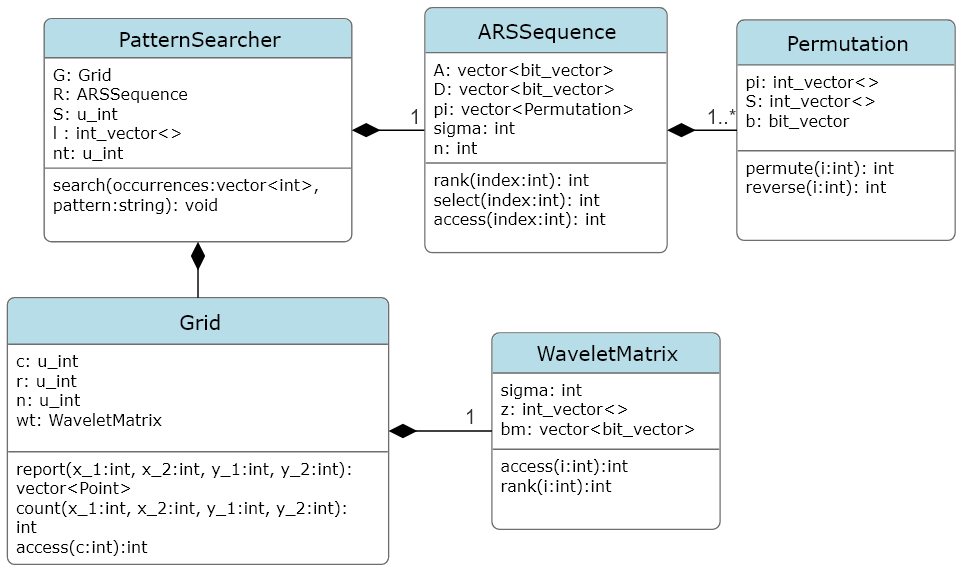
\includegraphics[width=1\textwidth]{imagenes/UML.png} % Adjust width as needed
    \label{fig:uml}
\end{figure}



\section{\textit{Re-Pair}}

La implementación de \textit{Re-Pair} de Shirou Maruyama\cite{re-pair} que utiliza las estrcuturas propuestas en la publicación original de Larsson \& Moffat\cite{Larsson2000}. Esta versión retorna una estructura que contiene un arreglo de reglas, además de la secuencia \textit{C} que corresponde a aquella que se obtiene una vez se aplican todas los reemplazos de las reglas en el texto original \textit{T}, y otros valores como la cantidad de reglas y el largo del texto (Véase \ref{lst:re-pair-call}). Las reglas corresponden a pares de enteros sin signo, donde los valores son menores a 256 si corresponden a una terminal o mayores si corresponden a una no terminal. Acceder a la posición 256 + $i$ del arreglo entrega la regla $i$.

\subsection{Generar reglas extras}
\label{sect:extrar}
Con objetivo de eliminar la secuencia \textit{C} para derivar el texto \textit{T} exclusivamente a partir de las reglas se crearon nuevas reglas $N_1 \rightarrow C[1] C[2]$, $N_2 \rightarrow C[3] C[4]$, $N_3 \rightarrow C[5] C[6]$, \textit{etc}, reemplazándolas en \textit{C}: $ N_1 N_2 N_3 ... N_{\lceil | C | /2 \rceil}$. Luego se hizo lo mismo con este nuevo \textit{C}, creando nuevas reglas $N^{'}_1 \rightarrow N_1 N_2$, $N^{'}_2 \rightarrow N_3 N_4$ y así sucesiva y recursivamente hasta obtener una única no terminal $S$ de la cual se puede derivar el texto original (Véase \ref{lst:rule-add}).

Sea $r = |\mathcal{R}|$ el número de reglas, y sea $A_i \rightarrow B_i C_i\; \forall\ 0\leq i < r$, el conjunto $\mathcal{R}$ es representado por la secuencia de enteros $R =  B_0 C_0 B_1 C_1 ... B_{r-1}C_{r-1}$. Nótese que la secuencia es auto-referencial: sea $R_i \rightarrow B_i C_i$, esta regla aparece en la secuencia en las posiciones $2i$ y $2i+1$, y reglas que deriven en $R_i$ tendrán uno de sus dos símbolos $B$ o $C$ con un valor 256 + $i$. 

Tómese en cuenta que en el trabajo presente cuando se habla de los lados izquierdo y derecho de una regla $R_i$, estos se refieren, respectivamente, a $B_i$ y $C_i$. También, cuando se hable de la compresión del texto a gramática, se hace referencia a la combinación de los procesos de comprimir por \textit{Re-Pair} seguido de la expansión de reglas con el fin de eliminar \textit{C}. 

La representación de la secuencia $R$, según las instrucciones del libro, utiliza permutaciones, y el detalle se explica más adelante, pero para hacer esta representación es necesario primero normalizar la secuencia de forma que los elementos en esta partan de 0 y sean continuos, es decir, el alfabeto de la secuencia no tiene saltos, y el mayor elemento es igual a la suma de las cantidades de terminales y no terminales menos 1.

\section{Normalizar secuencia}

Se creó un vector de bits \textit{b} (utilizando la librería \textit{SDSL}\cite{sdsl-lite}) de tamaño 256. La idea fue marcar con 1 las posiciones correspondientes a los símbolos terminales que aparecen en el texto \textit{T}, que son los símbolos terminales que aparecen en $R$. Esto conllevó a la restricción de que el texto debe tener formato donde cada carácter utiliza solo 1 byte (por ejemplo, UTF-8). Añadiendo suporte para \textit{Select}$_1$(\textit{i}) (reportar la posición del \textit{i}-ésimo uno en el vector) y \textit{Rank}$_1$(\textit{i}) (reportar la cantidad de unos hasta la posición \textit{i}) sobre el vector se puede obtener el símbolo original de la secuencia normalizada. Se guardan entonces los resultados de \textit{select} y \textit{rank} sobre el vector de bits, y estos dos vectores de largo 256 con elementos de tamaño 8 bits son los que se usarán en la estructura.

La secuencia normalizada ahora tiene símbolos entre 0 y la suma de las cantidades de terminales y no terminales menos 1. Elementos en la secuencia menores a la cantidad de terminales corresponden a símbolos terminales, mientras los demás corresponden a no terminales. La regla $R_i$ aparece en las posiciones $i$ y $i+1$ correspondiente a $B_i$ y $C_i$ respectivamente. Reglas que expanden a $R_i$ son las reglas $R_j$ donde alguno de sus $B_j$ o $C_j$ tienen como valor $i + $ número de terminales. El número de terminales es equivalente a \textit{rank}$_1$($b, |R|$). (Véase \ref{lst:normalizar})

Nótese que normalizar la secuencia es necesario solo para la implementación específica de \textit{Re-Pair} utilizada. En contraste, la versión de \textit{Re-Pair} de Navarro\cite{re-pair-navarro} normaliza automáticamente las reglas, entregando la secuencia \textit{C}, la secuencia \textit{R} de reglas, un valor numérico que indica la cantidad de símbolos terminales en el alfabeto usado en el texto y una secuencia numérica para obtener el símbolo original en el texto a partir del símbolo en la secuencia normalizada, exactamente como la implementación del trabajo presente.

\section{Secuencia utilizando permutaciones}

Se implementó la estructura descrita en el libro \cite[Capítulo~6.1]{Navarro} para representar secuencias de números utilizando permutaciones. Esta estructura permite las operaciones \textit{Access} y \textit{Rank} en tiempo $\mathcal{O}$(log log $\sigma$), donde $\sigma$ es el tamaño del alfabeto que compone la secuencia, y la operación \textit{Select} en tiempo $\mathcal{O}$(1). Esta última es importante pues es utilizada de forma frecuente en la búsqueda de ocurrencias secundarias en las reglas, lo cual será explicado más adelante.

\subsection{Permutaciones}

Una permutación $\pi$ de [1,n] es un reordenamiento de valores entre 1 y n. Descrita en el capítulo 5.1 \cite{Navarro}, la estructura que compete al trabajo realizado permite la operación $\pi^{-1}(i)$, esto es, la permutación inversa de $i$: encontrar un $j$ tal que $\pi(j) = i$ en tiempo $\mathcal{O}$(\textit{t}), donde \textit{t} es un parámetro de la estructura.

La idea de la estructura es aprovechar el concepto de descomposición en ciclos de la permutación. Si se aplica una permutación sobre un valor inicial se obtiene un segundo valor, y luego se aplica sobre este valor la permutación, y así sucesivamente, se terminará llegando al valor inicial. Este recorrido de valores se llama ciclo, y una permutación puede tener uno o más ciclos. 

Para calcular la permutación inversa de $i$ se aplica la permutación recursivamente hasta tener un $j$ cuya permutación es $i$. Esto requiere recorrer todo el ciclo que contiene a $i$. Sin embargo, si se guardan atajos de tamaño \textit{t}, con la idea de que si el elemento sobre el cual se está aplicando la permutación durante el recorrido del ciclo tiene un atajo, se toma ese atajo, saltándose una gran parte de los pasos recursivos, asegurando encontrar el inverso en no más de $t$ pasos.

Esta estructura se implemento satisfactoriamente utilizando los vectores de bit de la librería SDSL\cite{sdsl-lite} (Véase encabezado \ref{lst:perm}).

\subsection{Secuencia}

Dada la secuencia \textit{S} de tamaño \textit{n} sobre un alfabeto $\Sigma$, se divide esta, conceptualmente, en $\lceil n /\sigma \rceil$ pedazos $S_i = S[i \dots i+\sigma)$. Para resolver \textit{access}, \textit{rank} y \textit{select} se utilizan $\sigma$ vectores de bit $A_c$, con $c \in \Sigma$, donde $A_c = 1^{ rank_{c}(S_0, \sigma) } 0 1^{rank_{c}(S_1, \sigma)} \dots 0 1^{rank_{c}(S_{\lceil n /\sigma \rceil - 1}, \sigma)} $. En esencia, $A_c$ indica de forma unaria las ocurrencias del símbolo $c$ en casa pedazo de $S$. Con esto, las operaciones a nivel de los pedazos son:

Para todas $k = \lfloor i / \sigma \rfloor $.

\[ 
access(S, i) = access(S_k, i \ \text{mod} \ \sigma) 
\]
Para \textit{rank}, se debe calcular la cantidad de unos que aparecen en los pedazos anteriores al que corresponde a \textit{i}:
\[ 
rank_{c}(S, i) = 
\begin{cases} 
rank_{c}(S_k, i \ \text{mod} \ \sigma) & \text{si } k = 0,\\
rank_{c}(S_k, i \ \text{mod} \ \sigma) + select_{0}(A_{c}, k) - k & \text{si } k > 0
\end{cases} \]
Para \textit{select} se debe encontrar el pedazo al que pertenece el \textit{i} buscado, luego la respuesta es la suma de la posición donde parte este pedazo y \textit{select} sobre el pedazo, menos la posición del último cero antes del pedazo.
\[
select_{c}(S, j) = 
(s-j+1) \cdot \sigma +
select_{c}(S_{s-j+1}, s - \text{pred}_{0}(A_{c}, s)) \text{ donde } s = select_{1}(A_{c},j)
\]

Las operaciones dentro de cada pedazo \textit{C} requieren representar estos como la permutación inducida por su índice invertido. Sea $L_c$ la secuencia de las posiciones de los símbolos $c$ en el pedazo \textit{C}. Considérese la permutación $\pi = L_0 L_1 L_2 L_3 ... L_{\sigma-1}$ y las lista \textit{D} que marca las posiciones donde empieza cada lista en $\pi$, $D = 0^{|L_{0}|}10^{|L_{1}|} \dots 0^{|L_{\sigma-1}|}$

Utilizando la estructura anteriormente implementada se pueden resolver las operaciones dentro de los pedazos. Por ejemplo:

\[
access(C, i) = select_{0}(D, j) - j \text{, donde } j = \pi ^{-1}(i)
\]

Esta estructura se implementó correctamente (Véase el encabezado \ref{lst:seq})

\section{Reordenar secuencia}
\label{sec:reordenar}

La secuencia $R$ obtenida a partir de las reglas una vez completado el proceso de normalización es tal que estas reglas aparecen en el orden en que fueron creadas por el algoritmo \textit{Re-Pair} y extendidas con el fin de eliminar la secuencia \textit{C}. Lo que se quiere es que las reglas $R_i \rightarrow B_i C_i$ aparezcan ordenadas de forma creciente según el valor lexicográfico de la expansión inversa del lado izquierdo ($B_i$). 


La función de la librería estándar de C++ \textit{sort} puede ordenar la secuencia mientras se le otorgue una forma de expandir las reglas, pero esto no es suficiente pues se necesita que la secuencia de reglas mantenga la propiedad de auto-referencia, es decir, que cada regla $R_i$ aparezca en las posiciones $2i$ y $2i+1$ y que referencias a esta regla tenga el valor $i + \sigma$. Para lograr esto, se creó un vector de enteros que guarda los índices de cada regla. 

\begin{lstlisting}[style=cppstyle, caption={Vector de índices}, label={lst:example}]
int_vector reverseIndexMap(n_non_terminals);
for (int i = 0; i < n_non_terminals; i++) {
   reverseIndexMap[i] = i;
}
\end{lstlisting}

Luego se ordenó utilizando una función que compara las expansiones de los lados izquierdo de la regla apuntada por el índice, de forma inversa.
\begin{lstlisting}[style=cppstyle, caption={\textit{sort}}, label={lst:sort1}] 
sort(
    reverseIndexMap.begin(), 
    reverseIndexMap.end(), 
    [&](int a, int b) { 
        return compareRulesLazy(arsSequence, a, b, n_terminals, select, true); 
    }
);
\end{lstlisting}
La función de comparación es una función perezosa que entrega el siguiente símbolo de la expansión pedida a demanda, esto evita tener que expandir el lado requerido por completo, lo cual, en un texto largo con miles de reglas, puede llevar demasiado tiempo. Para esto se utilizaron generadores:

\begin{lstlisting}[style=cppstyle, caption={Comparación perezosa}, label={lst:cmp}] 
Generator<char> expandRuleSideLazy(
    ARSSequence& arrs, int i, int nt,
    std::vector<char>& sl, bool left = false)
{    
    int lr_i = left? i: i+1;
    if (arrs[lr_i] < nt) {
        co_yield sl[arrs[lr_i] + 1];
    } else {
        auto gen = expandRuleLazy(arrs, 2*(arrs[lr_i]-nt), nt, sl, left);
        for (char c : gen) {
            co_yield c;
        }
    }
}
bool compareRulesLazy(ARSSequence& arrs, int i, int j, int nt, std::vector<char>& sl, bool rev = false) 
{
    auto gen_i = expandRuleSideLazy(arrs, 2 * i, nt, sl, rev);
    auto gen_j = expandRuleSideLazy(arrs, 2 * j, nt, sl, rev);
    auto it_i = gen_i.begin();
    auto it_j = gen_j.begin();
    while (it_i != gen_i.end() && it_j != gen_j.end()) {
        char char_i = *it_i;
        char char_j = *it_j;
        if (char_i != char_j) {
            return char_i < char_j;
        }
        ++it_i;
        ++it_j;
    }
    // If one sequence is shorter, the shorter one is considered "less"
    return (it_i == gen_i.end()) && (it_j != gen_j.end());
}
\end{lstlisting}

Con esto, el vector \textit{reverseIndexMap} (rim) ahora contiene los índices de las reglas de forma tal que:
\[\forall i,j\ expansion\text{-}reversa (B_{rim[i]}) < expansion\text{-}reversa (B_{rim[i]})  \longleftrightarrow i < j \]
Se creó un vector del mismo tamaño que $R$ y se colocaron en este las reglas en el orden que aparecen en \textit{reverseIndexMap}, pero actualizando los valores $B$ y $C$:
\begin{lstlisting}[style=cppstyle, caption={\textit{Nueva secuencia R}}, label={lst:sort2}] 
vector<int> distance_of_find(reverseIndexMap.size(), 0);
for (int i = 0; i < reverseIndexMap.size(); i++) {
    distance_of_find[reverseIndexMap[i]] = i;        
}
int_vector<> sortedSequenceR = int_vector(n_non_terminals * 2 + 1, 0);
for (u_int i = 0; i < reverseIndexMap.size(); i++) {        
    int a_i = reverseIndexMap[i]; 
    int b_i = normalized_sequenceR[a_i*2];
    int c_i = normalized_sequenceR[a_i*2+1];
    int n_b_i, n_c_i;
    if (b_i < n_terminals) {
        n_b_i = b_i;
    } else {
        n_b_i = distance_of_find[b_i - n_terminals]  + n_terminals;
    }
    if (c_i < n_terminals) {
        n_c_i = c_i;
    } else {
        n_c_i = distance_of_find[c_i - n_terminals] + n_terminals;
    }
    sortedSequenceR[i*2] = n_b_i; 
    sortedSequenceR[i*2+1] = n_c_i; 
} 
int S_i = distance(reverseIndexMap.begin(), find(reverseIndexMap.begin(), reverseIndexMap.end(), n_non_terminals-1));  
sortedSequenceR[n_non_terminals*2] = S_i; 
R = ARSSequence(sortedSequenceR, max_normalized + 1 + 1);
\end{lstlisting}
La última linea guarda el índice de la regla inicial (anteriormente, la regla inicial era aquella expresada por los dos últimos valores en \textit{R}, ahora debe guardarse su posición).

Se creó también un vector similar a \textit{reverseIndexMap}, llamado \textit{indexMap} que guarda los índices de las reglas en el arreglo anteriormente ordenado, ordenadas por el valor lexicográfico de la expansión (no inversa) del lado derecho de cada regla. Este vector se utilizará para crear la grilla.

\subsection{Memoización}

Es posible aplicar la técnica de memoización para reducir el tiempo de la función de comparación, al guardar los valores de las expansiones de las reglas:

\begin{lstlisting}[style=cppstyle, caption={\textit{Nueva secuencia R}}, label={lst:sort3}] 
vector<int> distance_of_find(reverseIndexMap.size(), 0);
for (int i = 0; i < reverseIndexMap.size(); i++) {
    distance_of_find[reverseIndexMap[i]] = i;        
}
int_vector<> sortedSequenceR = int_vector(n_non_terminals * 2 + 1, 0);
for (u_int i = 0; i < reverseIndexMap.size(); i++) {        
    int a_i = reverseIndexMap[i]; 
    int b_i = normalized_sequenceR[a_i*2];
    int c_i = normalized_sequenceR[a_i*2+1];
    int n_b_i, n_c_i;
    if (b_i < n_terminals) {
        n_b_i = b_i;
    } else {
        n_b_i = distance_of_find[b_i - n_terminals]  + n_terminals;
    }
    if (c_i < n_terminals) {
        n_c_i = c_i;
    } else {
        n_c_i = distance_of_find[c_i - n_terminals] + n_terminals;
    }
    sortedSequenceR[i*2] = n_b_i; 
    sortedSequenceR[i*2+1] = n_c_i; 
} 
int S_i = distance(reverseIndexMap.begin(), find(reverseIndexMap.begin(), reverseIndexMap.end(), n_non_terminals-1));  
sortedSequenceR[n_non_terminals*2] = S_i; 
R = ARSSequence(sortedSequenceR, max_normalized + 1 + 1);
\end{lstlisting}

Esto sin embargo requiere mucho espacio extra y no comprime el texto, por lo que no es parte de la estructura, sin embargo posibles casos de utilidad son discutidos al final del trabajo.

\section{Ejemplo práctico}

Considérese el texto $T =$ \textit{abrabracadabrabra} y su versión normalizada:
\[T = 0\ 1\ 4\ 0\ 1\ 4\ 0\ 2\ 0\ 3\ 0\ 1\ 4\ 0\ 1\ 4\ 0
\]
Considérese también la gramática representada por la secuencia \textit{R}, normalizada y reordenada:
\[ R = 0\ 9\ 8\ 11\ 5\ 9\ 7\ 10\ 1\ 12\ 2\ 0\ 3\ 7\ 4\ 0  \] 
Donde la regla inicial es $R_1 = 8\ 11$.

Sea $s(i) = select_{1}(b, i + 1)$ ($b$ es el vector de bits obtenido durante la normalización de la secuencia) y $\sigma$ el tamaño del alfabeto de terminales (en este caso, con $\Sigma = $ [0, 1, 2, 3, 4] se tiene $\sigma = 5$), la figura \ref{fig:transformaciones} ilustra la expansión de las reglas, con $R_1$ la regla inicial que expande al texto original.
\begin{figure}[ht]
\centering

$R = 0\ 9\ 8\ 11\ 5\ 9\ 7\ 10\ 1\ 12\ 2\ 0\ 3\ 7\ 4\ 0$ \\
$(R = a R_4\ R_3 R_6\ R_0 R_4\ R_2 R_5\ b R_7\ c a\ d R_2\ r a)$
\[
\begin{array}{rl}
R_0 & \rightarrow 0\ 9 
\Longleftrightarrow s(0)\ R_{9 - \sigma} \Longleftrightarrow \textbf{a}\ R_{4} \Longleftrightarrow  \textbf{a} \text{ bra} \\
R_1 & \rightarrow 8\ 11\ 
\Longleftrightarrow R_{8 - \sigma}\ R_{11 - \sigma} \Longleftrightarrow R_{3}\ R_{6} \Longleftrightarrow \textbf{abrabraca} \text{ dabrabra} \\
R_2 & \rightarrow 5\ 9\ 
\Longleftrightarrow R_{5 - \sigma}\ R_{9 - \sigma} \Longleftrightarrow R_{0}\ R_{4} \Longleftrightarrow \textbf{abra} \text{ bra} \\
R_3 & \rightarrow 7\ 10\ 
\Longleftrightarrow R_{7 - \sigma}\ R_{10 - \sigma} \Longleftrightarrow R_{2}\ R_{5} \Longleftrightarrow \textbf{abrabra} \text{ ca} \\
R_4 & \rightarrow 1\ 12\ 
\Longleftrightarrow s(1)\ R_{12 - \sigma} \Longleftrightarrow \textbf{b}\ R_{7} \Longleftrightarrow \textbf{b} \text{ ra} \\
R_5 & \rightarrow 2\ 0\ 
\Longleftrightarrow s(2)\ s(0) \Longleftrightarrow \textbf{c} \text{ a} \\
R_6 & \rightarrow 3\ 7\ 
\Longleftrightarrow s(3)\ R_{7 - \sigma} \Longleftrightarrow \textbf{d}\ R_2 \Longleftrightarrow \textbf{d} \text{ abrabra} \\
R_7 & \rightarrow 4\ 0 
\Longleftrightarrow s(4)\ s(0) \Longleftrightarrow \textbf{r} \text{ a} \\
\end{array}
\]
$l = 4\ 17\ 7\ 9\ 3\ 2\ 8\ 2$
\caption{Secuencia \textit{R} y expansión de las reglas $R_i$, junto con secuencia \textit{l}, el largo de cada expansión}
\label{fig:transformaciones}
\end{figure}

Como se aprecia al expandir cada regla, estas están ordenadas de forma ascendente por el valor lexicográfico de la expansión invertida del lado izquierdo (en negrita).

Es posible visualizar esta gramática como un \textbf{árbol sintáctico} o \textit{parsing tree} (Véase figura \ref{fig:tree}) que se obtiene de recorrer \textit{R} desde la regla inicial $R_1$. Esta figura permite visualizar la idea de \textbf{Gramática Balanceada}: en una gramática balanceada, la altura del árbol sintáctico es del orden $\mathcal{O}(\log n)$, con \textit{n} es el largo del texto original, es decir, existe una constante \textit{c} tal que la altura es $\leq c \log n$ para todos los textos de largo \textit{n}. 

Para que la gramática representada por \textit{R} sea balanceada es menester que la implementación de \textit{Re-Pair} genere una gramática balanceada, luego la expansión de las reglas es balanceada naturalmente.

\begin{figure}[ht]
\centering
\begin{tikzpicture}[
    level distance=1.05cm, % Increases the vertical spacing
    level 1/.style={sibling distance=6cm}, % Adjust sibling spacing for top level
    level 2/.style={sibling distance=4cm},
    level 3/.style={sibling distance=3cm},
    level 4/.style={sibling distance=2cm},
    level 5/.style={sibling distance=2cm}, % Add specific spacing for deeper levels
    edge from parent/.style={draw, -latex}
]

% Root node
\node (R1) [circle, draw]{\( R_1 \)}
    child {node[circle, draw] {\( R_{3} \)}
        child {node[circle, draw] {\( R_2 \) }
            child {node[circle, draw]{\( R_0 \)}
                child {node{\( a \)}}
                    child {node[circle, draw]{\( R_4 \)}
                        child {node{\( b \)}}
                        child {node[circle, draw]{\( R_7 \)}
                            child {node{\( r \)}}
                            child {node{\( a \)}}
                        }
                    }
            }
            child {node[circle, draw]{\( R_4 \)}
                child {node{\( b \)}}
                child {node[circle, draw]{\( R_7 \)}
                    child {node{\( r \)}}
                    child {node{\( a \)}}
                }
            }
        }
        child {node[circle, draw] {\( R_5 \)}
            child {node {\( c \)  }}
            child {node {\( a \)  }}
        }
    }
    child {node[circle, draw] {\( R_6 \)}
        child {node {\( d \)   }}
        child {node[circle, draw] {\( R_2 \)  }
            child {node[circle, draw]{\( R_0 \)}
                child {node{\( a \)}}
                child {node[circle, draw]{\( R_4 \)}
                    child {node{\( b \)}}
                    child {node[circle, draw]{\( R_7 \)}
                        child {node{\( r \)}}
                        child {node{\( a \)}}
                    }
                }
            }
            child {node[circle, draw]{\( R_4 \)}
                child {node{\( b \)}}
                child {node[circle, draw]{\( R_7 \)}
                    child {node{\( r \)}}
                    child {node{\( a \)}}
                }
            }
        }
    };

\end{tikzpicture}
\caption{Árbol sintáctico para \textit{abrabracadabrabra}}
\label{fig:tree}
\end{figure}

Otra visualización de la gramática que será de utilidad para visualizar la búsqueda de patrones es la de un grafo acíclico dirigido o DAG (del inglés \textit{Directed Acyclic Graph}) (Fígura \ref{fig:DAG}). 

El DAG se forma de la siguiente forma. Cada regla tiene un único nodo correspondiente en el grafo. Cada vez que una regla $R_i$ aparece ya sea como lado izquierdo o derecho de otra regla $R_j$, esto induce una conexión desde el nodo $R_i$ al nodo $R_j$. El único nodo sin conexiones salientes corresponde a la regla inicial, en este caso, $R_1$.

\begin{figure}[H]
\begin{tikzpicture}[
	roundnode/.style={circle, draw=gray!100, thick, minimum size=6mm},
    squarenode/.style={rectangle, draw=gray!100, thick, minimum size=6mm},]
	
	\node[roundnode,font=\bfseries\sffamily] (R1) at (5.5,0) {$R_1$};
    
	\node[roundnode,font=\bfseries\sffamily] (R3) at (4,-0.9) {$R_3$};
	\node[roundnode,font=\bfseries\sffamily] (R6) at (7,-1) {$R_6$};
    
	\node[roundnode,font=\bfseries\sffamily] (R2) at (3,-2.3) {$R_2$};
    \node[roundnode,font=\bfseries\sffamily] (R5) at (5,-2.3) {$R_5$};
    \node[squarenode,font=\bfseries\sffamily] (d) at (6,-2.3) {$d$};

    \node[roundnode,font=\bfseries\sffamily] (R0) at (2,-3.5) {$R_0$};
    \node[roundnode,font=\bfseries\sffamily] (R4) at (3.4,-4.4) {$R_4$};
    \node[squarenode,font=\bfseries\sffamily] (c) at (4.1,-3.5) {$c$};

    \node[roundnode,font=\bfseries\sffamily] (R7) at (4.4,-5.8) {$R_7$};
    \node[squarenode,font=\bfseries\sffamily] (b) at (3.0,-5.8) {$b$};

    \node[squarenode,font=\bfseries\sffamily] (r) at (3.9,-7.0) {$r$};
    \node[squarenode,font=\bfseries\sffamily] (a) at (5.2,-7.0) {$a$};
	
	\draw [->, gray, -{Latex[length=1.5mm, width=2mm]}] (R3) to (R1);
    \draw [->, black, -{Latex[length=1.5mm, width=2mm]}] (R6) to (R1);
    
    \draw [->, gray, -{Latex[length=2mm, width=2mm]}] (R2) to (R3);
    \draw [->, black, -{Latex[length=1.5mm, width=2mm]}] (R5) to (R3);
    \draw [->, gray, -{Latex[length=2mm, width=2mm]}] (d) to (R6);  
    \draw [->, black, -{Latex[length=2mm, width=2mm]}] (R2) to[out=45, in=315] (R6);

    \draw [->, gray, -{Latex[length=2mm, width=2mm]}] (R0) to (R2);
    \draw [->, black, -{Latex[length=2mm, width=2mm]}] (R4) to[out=90, in=315] (R2);
    \draw [->, black, -{Latex[length=2mm, width=2mm]}] (R4) to (R0);
    \draw [->, gray, -{Latex[length=2mm, width=2mm]}] (c) to (R5);

    \draw [->, gray, -{Latex[length=2mm, width=2mm]}] (a) to[out=225, in=225] (R0);
    \draw [->, black, -{Latex[length=2mm, width=2mm]}] (a) to[out=30, in=315] (R5);
    \draw [->, black, -{Latex[length=2mm, width=2mm]}] (a) to (R7);
    \draw [->, gray, -{Latex[length=2mm, width=2mm]}] (r) to (R7);

    \draw [->, gray, -{Latex[length=2mm, width=2mm]}] (b) to (R4);
    \draw [->, black, -{Latex[length=2mm, width=2mm]}] (R7) to (R4);
	
	
\end{tikzpicture}
\caption{DAG para \textit{abrabracadabrabra}, las conexiones que corresponden a reglas que aparecen como lados izquierdos son grises, y las derechas son negras}
\label{fig:DAG}
\end{figure}


\newpage
\section{Grilla}

\textit{Compact Data Structures}\cite{Navarro} describe en su décimo capítulo la estructura de grilla en base a árboles \textit{wavelet} (más precisamente, las estructuras utilizan matrices \textit{wavelet}, pero los algoritmos descritos en el libro utilizan árboles). Para esto primero se ordenan los puntos de entrada por la coordenada \textit{x}. Luego, cada punto $(x_i, y_i)$ es representado en la grilla por el punto $(i, y_i)$. El mapeo entre los puntos originales y los nuevos se guarda en un vector de bits, sin embargo, esto es innecesario para el caso presente debido a que los valores $x_i$ son únicos y continuos, con lo cual al ordenar los puntos por \textit{x}, $(x_i, y_i) = (i, y_i)$. Una vez se tienen los puntos ordenados, si se consideran ahora solo los valores $y_i$ de cada punto, se tiene una secuencia \textit{S}. Es a partir de esta secuencia que se crea la matriz \textit{wavelet}\cite[Capítulo 6.2.5]{Navarro}.

\subsection{Matrices \textit{Wavelet}}

La idea de la matriz \textit{wavelet} es concatenar todos los vectores de bits en un mismo nivel para deshacerse de la topología de árbol. La forma particular en que son concatenados los vectores busca evitar espacios vacíos que aparecen en el árbol (pues no todos los caminos raíz-hoja tienen el mismo largo) es la siguiente: se colocan primero los vectores de bits correspondientes a hijos izquierdos del nivel anterior y luego los hijos derechos. Por ejemplo, para la secuencia "\textit{tobeornottobethatisthequestion}":

\[
\begin{array}{lcll}
S_1 & : & \texttt{tobeornottobethatisthequestion} & \\
B_1 & : & \texttt{110011011110010010110011011010} & z_1 = 13 \\[10pt]
S_2 & : & \texttt{benbehaiheein toorottottstqusto} & \\
B_2 & : & \texttt{0010010110011 10000110111101110} & z_2 = 14 \\[10pt]
S_3 & : & \texttt{bebeaee oorooqo nhihin tttttstust } & \\
B_3 & : & \texttt{0101011 0010000 100001 0000000100 } & z_3 = 22 \\[10pt]
S_4 & : & \texttt{bba ooooqo hihi tttttstst eeee r nn u} & \\
B_4 & : & \texttt{110 000010 0101 111110101 } & z_4 = 10 \\[10pt]
S_5 & : & \texttt{a ooooo hh ss bb q ii ttttttt} & \\
\end{array}
\]

Donde $z_l$ es un valor pre-calculado equivalente a $Rank_0 (B_{l}, n)$.

La estructura y sus operaciones se implementaron correctamente (Véase \ref{lst:wlmt}) siguiendo las instrucciones del capítulo 6.2.5 de \textit{Compact Data Structures}\cite{Navarro}. Con esto, se implementó la estructura de grilla usando matrices \textit{wavelet}\cite[Capítulo 10.1]{Navarro} (Véase \ref{lst:grid}).

\subsection{Preparar puntos para grilla}

Cada regla $R_i \rightarrow B_i C_i $ se guarda en la grilla en un punto con coordenadas $(B_i, C_i)$. Las filas de la grilla están ordenadas por orden lexicográfico del reverso de la expansión de $B_i$ (esto ya se hizo). Las columnas en tanto están ordenadas por orden lexicográfico de la expansión de $C_i$. Para lograr esto se usó el vector \textit{indexMap} descrito previamente:
\begin{lstlisting}[style=cppstyle] 
std::vector<Point> points(n_non_terminals);
u_int j, k;
for (u_int i = 0; i < indexMap.size(); i++) {
    k = std::distance(indexMap.begin(), std::find(indexMap.begin(), indexMap.end(), i));
    points[i] = Point(k, i);
}    
\end{lstlisting}

Estos puntos se usaron para inicializar la grilla (La implementación de la grilla usa valores indexados desde 1, por lo que hay que sumar 1 a los valores de los puntos antes de usarlos).

Por ejemplo, las reglas generadas por "\textit{abrabracadabrabra}" (Véase la fígura \ref{fig:transformaciones}), conforman la siguiente grilla:

\begin{figure}[h]
    \centering
    \begin{tikzpicture}[scale=0.7]% Draw the grid
	\draw[step=1cm,gray,opacity=0.5] (0,0) grid (7,7);	
	\node[anchor=north west,rotate=90] at (0-0.3, 7.5) {a};
	\node[anchor=north west,rotate=90] at (1-0.3, 7.5) {a};
	\node[anchor=north west,rotate=90] at (2-0.4, 7.5) {abrara};
	\node[anchor=north west,rotate=90] at (3-0.4, 7.5) {bra};
	\node[anchor=north west,rotate=90] at (4-0.38, 7.5) {bra};
	\node[anchor=north west,rotate=90] at (5-0.35, 7.5) {ca};
	\node[anchor=north west,rotate=90] at (6-0.35, 7.5) {dabrabra};
	\node[anchor=north west,rotate=90] at (7-0.3, 7.5) {ra};	
	\node[anchor=north east] at (-0.5,7+0.3) {a};
	\node[anchor=north east] at (-0.5,6+0.4) {abrabraca};
	\node[anchor=north east] at (-0.5,5+0.4) {abra};
	\node[anchor=north east] at (-0.5,4+0.4) {abrabra};
	\node[anchor=north east] at (-0.5,3+0.4) {b};
	\node[anchor=north east] at (-0.5,2+0.4) {c};
	\node[anchor=north east] at (-0.5,1+0.5) {d};
	\node[anchor=north east] at (-0.5,0+0.4) {r};
	%\pattern[pattern=north west lines, pattern color=gray] (0.0-0.2,4.0-0.3) rectangle (7.0+0.2,7.0+0.3);
	%\draw[red, thick] (0.0-0.2,4.0-0.3) rectangle (7.0+0.2,7.0+0.3);
	
	%\pattern[pattern=north east lines, pattern color=gray] (3.0-0.2,0.0-0.3) rectangle (4.0+0.3,7.0+0.4);
	%\draw[blue, thick] (3.0-0.3,0.0-0.3) rectangle (4.0+0.3,7.0+0.4);	
	\node[anchor=south west, text=black, font=\bfseries\sffamily] at (0.0-0.4,2.0-0.4) {$R_5$};
	\node[anchor=south west, text=black, font=\bfseries\sffamily] at (1.0-0.4,0.0-0.4) {$R_7$};
	\node[anchor=south west, text=black, font=\bfseries\sffamily] at (2.0-0.4,1.0-0.4) {$R_6$};
	\node[anchor=south west, text=black, font=\bfseries\sffamily] at (3.0-0.4,7.0-0.4) {$R_0$};
	\node[anchor=south west, text=black, font=\bfseries\sffamily] at (4.0-0.4,5.0-0.4) {$R_2$};
	\node[anchor=south west, text=black, font=\bfseries\sffamily] at (5.0-0.4,4.0-0.4) {$R_3$};
	\node[anchor=south west, text=black, font=\bfseries\sffamily] at (6.0-0.4,6.0-0.4) {$R_1$};
	\node[anchor=south west, text=black, font=\bfseries\sffamily] at (7.0-0.45,3.0-0.4) {$R_4$};
    
    \node[anchor=south west, text=black, font=\bfseries\sffamily] at (0-0.4,-1-0.5) {0};
    \node[anchor=south west, text=black, font=\bfseries\sffamily] at (1-0.4,-1-0.5) {1};
    \node[anchor=south west, text=black, font=\bfseries\sffamily] at (2-0.4,-1-0.5) {2};
    \node[anchor=south west, text=black, font=\bfseries\sffamily] at (3-0.4,-1-0.5) {3};
    \node[anchor=south west, text=black, font=\bfseries\sffamily] at (4-0.4,-1-0.5) {4};
    \node[anchor=south west, text=black, font=\bfseries\sffamily] at (5-0.4,-1-0.5) {5};
    \node[anchor=south west, text=black, font=\bfseries\sffamily] at (6-0.4,-1-0.5) {6};
    \node[anchor=south west, text=black, font=\bfseries\sffamily] at (7-0.4,-1-0.5) {7};
\end{tikzpicture}
    
    \caption{Grilla}
    \label{fig:grid}
\end{figure}


Si se lee la grilla fila por fila aparecen las reglas en este orden: $R_0, R_1, R_2, ... R_7$, es decir, en el orden preexistente, pues ya fueron ordenadas por orden lexicográfico de la expansión reversa del lado izquierdo (mostrado en la figura a la izquierda de cada fila). Si se leen las reglas columna a columna, el orden es $R_5, R_7, R_6, R_0, R_2, R_3, R_1, R_4$, pues las columnas están ordenadas por orden lexicográfico de la expansión del lado derecho (mostrado arriba de la grilla sobre cada columna correspondiente).

\section{Calcular largo de las expansiones de las reglas}

Es menester, para poder responder consultas de búsqueda de patrones, pre-calcular los valores de los largos de las expansiones de cada regla. El detalle se ve más adelante, pero en resumen, si una ocurrencia de un patrón sucede en una regla que aparece como el lado derecho $C_i$ de otra regla, el índice del patrón estará desfasado $l_{B_i}$ con respecto al índice de la regla padre, donde $l_{B_i}$ es el largo de la expansión de la regla $B_i$ que es el lado izquierdo de la regla $R_i$. 

\begin{lstlisting}[style=cppstyle]
l = int_vector(n_non_terminals, 0); // largos de cada regla
for (int i = 0; i < n_non_terminals; i++) {
    l[i] = ruleLength(i);
}
\end{lstlisting}

Como las reglas son referenciadas por otras reglas (y dependiendo de lo repetitivo del texto, son referenciadas más de una vez), con el fin de evitar calcular el largo para una misma regla cada vez que esta es parte de la expansión de otra, se usó \textit{memoización} (en este caso, la misma lista de largos funciona como la memoria).

\begin{lstlisting}[style=cppstyle]
int PatternSearcher::ruleLength(int_vector<> *l, int i) {
    if (l[i] != 0) { //memoization
        return l[i];
    }
    int left, right;
    if (R[i*2] < nt) {
        left = 1;
    } else {
        left = ruleLength(R[i*2] - nt);
    }
    if (R[i*2+1] < nt) {
        right = 1;
    } else {
        right = ruleLength(R[i*2+1] - nt);
    }
    l[i] = left + right;
    return l[i];
}
\end{lstlisting}

\section{Búsqueda de patrones}

La búsqueda de patrones aprovecha la grilla para encontrar las reglas en las que aparece el patrón de texto buscado. La idea es la siguiente: si el patrón $P$ a buscar aparece en el texto, entonces existe al menos una división del patrón $P$ en dos \textit{strings} $P_<$ y $P_>$ que son prefijo y sufijo del patrón respectivamente y que concatenados forman el patrón $P$, tales que $P_<$ es sufijo de la expansión izquierda de una regla $R_i$ y $P_>$ es prefijo de la expansión derecha de la misma regla. Si se tienen todas las reglas que cumplen esta condición, basta con recorrer virtualmente el árbol sintáctico o \textit{parsing tree} hasta el símbolo inicial, y entregar la posición donde parte $P_<$ tomando en cuenta los desfases con respecto al nodo padre. 

La idea entonces es, primero, y por cada división $P_<$ y $P_>$ del patrón, encontrar todas la reglas que expresan el patrón de la forma descrita (ocurrencias primarias), y luego, por cada una de estas reglas encontradas, hacer accesos en \textit{R} hasta encontrar todas las posiciones de esta regla en el símbolo inicial (ocurrencias secundarias). El detalle se ve en las siguientes secciones.

\subsection{Ocurrencias primarias}

Para cada posible división del patrón \textit{P} en dos \textit{strings}, uno prefijo y otro sufijo $P_<$ y $P_>$, se buscan las reglas cuya expansión izquierda es $P_<$ y derecha $P_>$.

Como las filas están ordenadas por orden lexicográfico de la expansión reversa del lado izquierdo de estas, las reglas que cuyo lado izquierdo terminan en $P_<$ forman un rango de filas en la grilla. De forma análoga, las columnas están ordenadas de forma lexicográfica por la expansión del lado derecho, por lo que las reglas con lado derecho que empieza con $P_>$ forman un rango de columnas. Esto significa que se puede encontrar el rango de filas y columnas (y por lo tanto, el cuadrante donde se encuentran las reglas que cumplen con la condición buscada) usando búsqueda binaria.

Por ejemplo, sea el patrón de búsqueda $P =$ \textbf{ab} sobre el texto \textit{abrabracadabrabra}, se tienen los posibles (y en este caso únicos) $P_< =$ \textbf{a} y $P_> =$ \textbf{b}. Las reglas que tienen como sufijo en su extensión izquierda a $P_< =$ \textbf{a} están en el rango de filas [$0,1,2,3$] (en ázul en la figura \ref{fig:grid-2}), mientras que las reglas que tienen como prefijo en el lado derecho a $P_> =$ \textbf{b} están en el rango de columnas [$3, 4$] (en rojo en la figura \ref{fig:grid-2}).

\begin{figure}[h]
    \centering
    \begin{tikzpicture}[scale=0.7]% Draw the grid
	\draw[step=1cm,gray,opacity=0.5] (0,0) grid (7,7);	
	\node[anchor=north west,rotate=90] at (0-0.3, 7.5) {a};
	\node[anchor=north west,rotate=90] at (1-0.3, 7.5) {a};
	\node[anchor=north west,rotate=90] at (2-0.4, 7.5) {abrara};
	\node[anchor=north west,rotate=90] at (3-0.4, 7.5) {bra};
	\node[anchor=north west,rotate=90] at (4-0.38, 7.5) {bra};
	\node[anchor=north west,rotate=90] at (5-0.35, 7.5) {ca};
	\node[anchor=north west,rotate=90] at (6-0.35, 7.5) {dabrabra};
	\node[anchor=north west,rotate=90] at (7-0.3, 7.5) {ra};	
	\node[anchor=north east] at (-0.5,7+0.3) {a};
	\node[anchor=north east] at (-0.5,6+0.4) {abrabraca};
	\node[anchor=north east] at (-0.5,5+0.4) {abra};
	\node[anchor=north east] at (-0.5,4+0.4) {abrabra};
	\node[anchor=north east] at (-0.5,3+0.4) {b};
	\node[anchor=north east] at (-0.5,2+0.4) {c};
	\node[anchor=north east] at (-0.5,1+0.5) {d};
	\node[anchor=north east] at (-0.5,0+0.4) {r};
	\pattern[pattern=north west lines, pattern color=blue, opacity=0.5] (0.0-0.2,4.0-0.3) rectangle (7.0+0.2,7.0+0.3);
	%\draw[red, thick] (0.0-0.2,4.0-0.3) rectangle (7.0+0.2,7.0+0.3);
	
	\pattern[pattern=north east lines, pattern color=red, opacity=0.5] (3.0-0.2,0.0-0.3) rectangle (4.0+0.3,7.0+0.4);
	%\draw[blue, thick] (3.0-0.3,0.0-0.3) rectangle (4.0+0.3,7.0+0.4);	
	\node[anchor=south west, text=black, font=\bfseries\sffamily] at (0.0-0.4,2.0-0.4) {$R_5$};
	\node[anchor=south west, text=black, font=\bfseries\sffamily] at (1.0-0.4,0.0-0.4) {$R_7$};
	\node[anchor=south west, text=black, font=\bfseries\sffamily] at (2.0-0.4,1.0-0.4) {$R_6$};
	\node[anchor=south west, text=black, font=\bfseries\sffamily] at (3.0-0.4,7.0-0.4) {$R_0$};
	\node[anchor=south west, text=black, font=\bfseries\sffamily] at (4.0-0.4,5.0-0.4) {$R_2$};
	\node[anchor=south west, text=black, font=\bfseries\sffamily] at (5.0-0.4,4.0-0.4) {$R_3$};
	\node[anchor=south west, text=black, font=\bfseries\sffamily] at (6.0-0.4,6.0-0.4) {$R_1$};
	\node[anchor=south west, text=black, font=\bfseries\sffamily] at (7.0-0.45,3.0-0.4) {$R_4$};
    
    \node[anchor=south west, text=black, font=\bfseries\sffamily] at (0-0.4,-1-0.5) {0};
    \node[anchor=south west, text=black, font=\bfseries\sffamily] at (1-0.4,-1-0.5) {1};
    \node[anchor=south west, text=black, font=\bfseries\sffamily] at (2-0.4,-1-0.5) {2};
    \node[anchor=south west, text=black, font=\bfseries\sffamily] at (3-0.4,-1-0.5) {3};
    \node[anchor=south west, text=black, font=\bfseries\sffamily] at (4-0.4,-1-0.5) {4};
    \node[anchor=south west, text=black, font=\bfseries\sffamily] at (5-0.4,-1-0.5) {5};
    \node[anchor=south west, text=black, font=\bfseries\sffamily] at (6-0.4,-1-0.5) {6};
    \node[anchor=south west, text=black, font=\bfseries\sffamily] at (7-0.4,-1-0.5) {7};
\end{tikzpicture}
    
    \caption{Grilla}
    \label{fig:grid-2}
\end{figure}

Las reglas $R_0$ y $R_2$ se encuentran en el cuadrante definido por los dos rangos encontrados. Estas reglas pueden obtenerse mediante la operación \textit{report} de la grilla. El siguiente paso es determinar los índices de las reglas en el texto original (Véase sección \ref{sect:second}). 

\subsubsection{Implementación}

La búsqueda de las reglas que contienen el patrón consiste en primero dividir este en dos \textit{sub-strings} ($P_<, P_>$), según una variable \textit{t} (el largo de $P_<$). Por cada \textit{t} entre 1 y el largo del patrón menos uno, se deben encontrar $s_y$ (primera fila del rango de filas), $e_y$ (última fila del rango), $s_x$ (primera columna del rango de columnas) y $e_x$ (última columna del rango).

\begin{lstlisting}[style=cppstyle]
u_int m = P.size();
u_int t;
for (t = 1; t < m; t++) {
    string P_left = P.substr(0, t); // P_<
    string P_right = P.substr(t, m-t); // P_>
    uint s_x, e_x, s_y, e_y;
\end{lstlisting}

Para buscar los rangos $s_x, e_x, s_y, e_y$ , se utilizó búsqueda binaria, como se ve en \ref{lst:search}, donde se muestra la búsqueda binaria para $s_y$. En este caso, la fila tiene el mismo identificador que la regla (línea 5) gracias a la disposición de los puntos usados en la grilla.

\begin{lstlisting}[style=cppstyle, caption={Búsqueda binaria para $s_y$}, label={lst:search}]
int left = 0, right = G.getRows() - 1;
int result = -1;
while (left <= right) {
    int mid = left + (right - left) / 2;
    int r_i = mid;
    int compare = compareRuleWithPatternLazy(R, r_i, nt, sl, P_left, true);
    if (compare >= 0) { 
        if (compare == 0) 
            result = mid;      
        right = mid - 1;
    } else {
        left = mid + 1;
    }
}
if (result == -1) continue;
s_y = result + 1; 
\end{lstlisting}

En el caso de las columnas, la línea 5 de \ref{lst:search} debe cambiar, el índice de la regla corresponde al valor del punto en la columna:
\begin{lstlisting}[style=cppstyle]
int r_i = G.access(mid+1)-1; // rule index
\end{lstlisting}
Donde $G.access$ entrega el valor del único punto en la columna de entrada. 

Para encontrar el final de cada rango, lo único que cambia en la búsqueda binaria es como se mueven los límites de la búsqueda (\textit{left} y \textit{right}):
\begin{lstlisting}[style=cppstyle]
    if (compare <= 0) {
        if (compare == 0) {
            result = mid;
        }
        left = mid + 1; // instead of mid - 1
    } else {
        right = mid - 1; // instead of mid + 1
    }
\end{lstlisting}

La función \textit{compareRuleWithPatternLazy} compara el patrón con la expansión ya sea izquierda o derecha de una regla, como se ve en \ref{lst:patterncompare}.

\begin{lstlisting}[style=cppstyle, caption={Ocurrencias}, label={lst:patterncompare}]
template <typename Iterator>
int compareRuleWithPatternLazyImpl(
    ARSSequence& arrs, int i, int nt, std::vector<char>& sl, Iterator pattern_begin, Iterator pattern_end,
    bool rev = false) 
{      
    auto gen = expandRuleSideLazy(arrs, 2*i, nt, sl, rev);
    auto it = gen.begin();
    while (it != gen.end() && pattern_begin != pattern_end) {
        char c = *it;
        char p = *pattern_begin;
        if (c < p) return -1; 
        if (c > p) return 1;  
        ++it;
        ++pattern_begin;
    }
    if (it == gen.end() && pattern_begin != pattern_end) return -1; 
    return 0; 
}
int compareRuleWithPatternLazy(ARSSequence& arrs, int i, int nt, std::vector<char>& sl, std::string pattern, bool rev = false) 
    {  
    if (rev) {
        return compareRuleWithPatternLazyImpl(arrs, i, nt, sl, pattern.rbegin(), pattern.rend(), rev);
    } else {
        return compareRuleWithPatternLazyImpl(arrs, i, nt, sl, pattern.begin(), pattern.end(), rev);
    }
}
\end{lstlisting}

Esta operación utiliza las funciones de expansión perezosa descritas en la sección \ref{sec:reordenar}, en el fragmento \ref{lst:cmp}.

Una vez encontrados los rangos, se deben encontrar las ocurrencias de las reglas que se encuentran en este:

\begin{lstlisting}[style=cppstyle]
vector<Point> points = G.report(s_x, e_x, s_y, e_y); 
for (Point p: points) {
    int r_i = p.second-1; // rule index
    if ((u_int)R[r_i*2] < nt) { 
        secondaries(occurences, R, S, r_i, nt, l, 0);
    } else {
        secondaries(occurences, R, S, r_i, nt, l, l[R[r_i*2] - nt]-t);
    }
}
\end{lstlisting}
El desfase inicial es cero si el lado izquierdo es una terminal, en el caso contrario el desfase es la diferencia entre el largo de la expansión del lado izquierdo y el largo de $P_<$.

\subsection{Ocurrencias secundarias }
\label{sect:second}
Determinar las posiciones de las reglas encontradas en el símbolo inicial corresponde a recorrer virtualmente el DAG desde los nodos correspondientes a cada regla encontrada en la búsqueda de ocurrencias primarias hasta el nodo correspondiente al símbolo inicial, acumulando el desfase de cada nodo en el camino: si la regla es el hijo derecho del nodo destino, su desfase respecto a este es igual al largo de la expansión de la correspondiente regla izquierda. 

La idea es recorrer todos los caminos posibles hasta el nodo inicial, y entregar los desfases para cada recorrido. 

\begin{figure}[H]
\begin{tikzpicture}[
	roundnode/.style={circle, draw=gray!100, thick, minimum size=6mm},
    squarenode/.style={rectangle, draw=gray!100, thick, minimum size=6mm},]
	
	\node[roundnode,font=\bfseries\sffamily] (R1) at (5.5,0) {$R_1$};
    
	\node[roundnode,font=\bfseries\sffamily] (R3) at (4,-0.9) {$R_3$};
	\node[roundnode,font=\bfseries\sffamily] (R6) at (7,-1) {$R_6$};
    
	\node[roundnode,font=\bfseries\sffamily] (R2) at (3,-2.3) {$R_2$};
    \node[roundnode,font=\bfseries\sffamily] (R5) at (5,-2.3) {$R_5$};
    \node[squarenode,font=\bfseries\sffamily] (d) at (6,-2.3) {$d$};

    \node[roundnode,font=\bfseries\sffamily] (R0) at (2,-3.5) {$R_0$};
    \node[roundnode,font=\bfseries\sffamily] (R4) at (3.4,-4.4) {$R_4$};
    \node[squarenode,font=\bfseries\sffamily] (c) at (4.1,-3.5) {$c$};

    \node[roundnode,font=\bfseries\sffamily] (R7) at (4.4,-5.8) {$R_7$};
    \node[squarenode,font=\bfseries\sffamily] (b) at (3.0,-5.8) {$b$};

    \node[squarenode,font=\bfseries\sffamily] (r) at (3.9,-7.0) {$r$};
    \node[squarenode,font=\bfseries\sffamily] (a) at (5.2,-7.0) {$a$};
	
	\draw [->, red, -{Latex[length=1.5mm, width=2.5mm]}] (R3) to (R1);
    \draw [->, blue, -{Latex[length=1.5mm, width=2.5mm]}] (R6) to (R1);
    
    \draw [->, red, -{Latex[length=2mm, width=2.5mm]}] (R2) to (R3);
    \draw [->, black, -{Latex[length=1.5mm, width=2mm]}] (R5) to (R3);
    \draw [->, gray, -{Latex[length=2mm, width=2mm]}] (d) to (R6);  
    \draw [->, blue, -{Latex[length=2mm, width=2.5mm]}] (R2) to[out=45, in=315] (R6);

    \draw [->, red, -{Latex[length=2mm, width=2.5mm]}] (R0) to[out=62, in=220] (R2);
    \draw [->, blue, -{Latex[length=2mm, width=2.5mm]}] (R0) to[out=59, in=222] (R2);
    \draw [->, black, -{Latex[length=2mm, width=2mm]}] (R4) to[out=90, in=315] (R2);
    \draw [->, black, -{Latex[length=2mm, width=2mm]}] (R4) to (R0);
    \draw [->, gray, -{Latex[length=2mm, width=2mm]}] (c) to (R5);

    \draw [->, gray, -{Latex[length=2mm, width=2mm]}] (a) to[out=225, in=225] (R0);
    \draw [->, black, -{Latex[length=2mm, width=2mm]}] (a) to[out=30, in=315] (R5);
    \draw [->, black, -{Latex[length=2mm, width=2mm]}] (a) to (R7);
    \draw [->, gray, -{Latex[length=2mm, width=2mm]}] (r) to (R7);

    \draw [->, gray, -{Latex[length=2mm, width=2mm]}] (b) to (R4);
    \draw [->, black, -{Latex[length=2mm, width=2mm]}] (R7) to (R4);
	
	
\end{tikzpicture}
\caption{Búsqueda en el DAG para nodo $R_0$}
\label{fig:DAG-search}
\end{figure}

Siguiendo el ejemplo de la sección anterior, se necesita ahora encontrar las ocurrencias de las reglas $R_0$ y $R_2$ en el texto, considerando el desfase inicial del patrón $P = \textbf{ab}$ con respecto a cada regla.

La figura \ref{fig:DAG-search} muestra el recorrido por el DAG que corresponde a la búsqueda de ocurrencias secundarias para el patrón $P = \textbf{ab}$ expresado en $R_0 = \textbf{a}\ \textbf{b}ra$.  Los dos caminos posibles (en rojo y ázul) llegan cada uno a $R_1$ con distintos desfases. El camino rojo llega con un desfase acumulado de 0 (el desfase inicial es 0 pues el patrón coincide con el inicio de la regla), lo que indica que el patrón (expresado por la regla $R_0$) aparece en la posición 0 del texto (indexado desde cero). El camino azul acumula un desfase igual a $l[d] + l[R_3] = 1 + 9 = 10$ (Véase figura \ref{fig:transformaciones} para los valores de \textit{l}), con lo que el patrón (en la regla $R_0$) aparece también en la posición 10 del texto. 

Considere ahora la búsqueda para la regla $R_2$. La fígura \ref{fig:DAG-search2} muestra los recorridos realizados por la búsqueda.

\begin{figure}[H]
\begin{tikzpicture}[
	roundnode/.style={circle, draw=gray!100, thick, minimum size=6mm},
    squarenode/.style={rectangle, draw=gray!100, thick, minimum size=6mm},]
	
	\node[roundnode,font=\bfseries\sffamily] (R1) at (5.5,0) {$R_1$};
    
	\node[roundnode,font=\bfseries\sffamily] (R3) at (4,-0.9) {$R_3$};
	\node[roundnode,font=\bfseries\sffamily] (R6) at (7,-1) {$R_6$};
    
	\node[roundnode,font=\bfseries\sffamily] (R2) at (3,-2.3) {$R_2$};
    \node[roundnode,font=\bfseries\sffamily] (R5) at (5,-2.3) {$R_5$};
    \node[squarenode,font=\bfseries\sffamily] (d) at (6,-2.3) {$d$};

    \node[roundnode,font=\bfseries\sffamily] (R0) at (2,-3.5) {$R_0$};
    \node[roundnode,font=\bfseries\sffamily] (R4) at (3.4,-4.4) {$R_4$};
    \node[squarenode,font=\bfseries\sffamily] (c) at (4.1,-3.5) {$c$};

    \node[roundnode,font=\bfseries\sffamily] (R7) at (4.4,-5.8) {$R_7$};
    \node[squarenode,font=\bfseries\sffamily] (b) at (3.0,-5.8) {$b$};

    \node[squarenode,font=\bfseries\sffamily] (r) at (3.9,-7.0) {$r$};
    \node[squarenode,font=\bfseries\sffamily] (a) at (5.2,-7.0) {$a$};
	
	\draw [->, red, -{Latex[length=1.5mm, width=2.5mm]}] (R3) to (R1);
    \draw [->, blue, -{Latex[length=1.5mm, width=2.5mm]}] (R6) to (R1);
    
    \draw [->, red, -{Latex[length=2mm, width=2.5mm]}] (R2) to (R3);
    \draw [->, black, -{Latex[length=1.5mm, width=2mm]}] (R5) to (R3);
    \draw [->, gray, -{Latex[length=2mm, width=2mm]}] (d) to (R6);  
    \draw [->, blue, -{Latex[length=2mm, width=2.5mm]}] (R2) to[out=45, in=315] (R6);

    \draw [->, gray, -{Latex[length=2mm, width=2mm]}] (R0) to (R2);
    \draw [->, black, -{Latex[length=2mm, width=2mm]}] (R4) to[out=90, in=315] (R2);
    \draw [->, black, -{Latex[length=2mm, width=2mm]}] (R4) to (R0);
    \draw [->, gray, -{Latex[length=2mm, width=2mm]}] (c) to (R5);

    \draw [->, gray, -{Latex[length=2mm, width=2mm]}] (a) to[out=225, in=225] (R0);
    \draw [->, black, -{Latex[length=2mm, width=2mm]}] (a) to[out=30, in=315] (R5);
    \draw [->, black, -{Latex[length=2mm, width=2mm]}] (a) to (R7);
    \draw [->, gray, -{Latex[length=2mm, width=2mm]}] (r) to (R7);

    \draw [->, gray, -{Latex[length=2mm, width=2mm]}] (b) to (R4);
    \draw [->, black, -{Latex[length=2mm, width=2mm]}] (R7) to (R4);
	
	
\end{tikzpicture}
\caption{Búsqueda en el DAG para nodo $R_2$}
\label{fig:DAG-search2}
\end{figure}

El camino rojo llega con un desfase acumulado de 3 (el desfase inicial del patrón $P = \textbf{ab}$ respecto a la regla $R_2 = abr\textbf{a}\ \textbf{b}ra$), mientras que el camino azul llega con un desfase $3 + l[d] + l[R_3] = 3 + 1 + 9 = 13$. Con esto se concluye que el patrón aparece (expresado en la regla $R_2$) en las posiciones 3 y 14. En total, sumando a las ocurrencias encontradas para $R_0$, el patrón aparece en las posiciones 0, 3, 10 y 14 del texto.

En este ejemplo, solo se necesitó encontrar un cuadrante, pues solo existía un par ($P_<$, $P_>$) para dividir \textbf{ab}, pero un patrón más largo tiene múltiples divisiones, por lo que para cada par ($P_<$, $P_>$) que tengan un cuadrante en la grilla válido se debe hacer el proceso de encontrar las ocurrencias secundarias.

\subsubsection{Implementación}
 
La búsqueda de ocurrencias secundarias en la implementación consiste en acceder \textit{R} de forma recursiva. La idea es la siguiente, en cada recursión, para una regla $R_k$ y un desfase acumulado se buscan todas las ocurrencias de la regla en \textit{R} (la cantidad de ocurrencias es dada por $r = rank (R, R_k)$, y cada ocurrencia $j \leq r$ está en $i =$ \textit{select}($R, R_{k}, j$)), y por cada una de estas, si la ocurrencia corresponde a un hijo derecho (es decir, si la posición \textit{i} de la \textit{j}-ésima $R_k$ en \textit{R} es impar) entonces se agrega al desfase acumulado el largo de la regla en la posición $i-1$. Seguido de esto se llama la búsqueda de ocurrencias secundarias para la regla $R_{i/2}$ que es la que contiene esta ocurrencia específica \textit{j} de $R_k$ en \textit{R}, es decir, es el nodo padre en el árbol sintáctico, con el desfase acumulado. La implementación de esto se ve en el fragmento \ref{lst:second}. Cada vez que se llega al símbolo inicial \textit{S} el desfase será distinto, correspondiente a cada índice del patrón buscado en el texto.

\begin{lstlisting}[style=cppstyle, caption={Ocurrencias}, label={lst:second}]
void secondaries(vector<int> *occs, ARSSequence R, u_int S,
    u_int A_i, u_int nt, int_vector<> l, u_int offset=0,
    bool terminal = false) {
    if (!terminal && A_i == S) { 
        occs->push_back(offset); return;
    }
    int c = terminal? A_i: A_i + nt; // nt = number of terminals
    for (int j=1; j <= R.rank(c, R.size()); j++) {
        int k = R.select(c, j);
        int D_i = k / 2;
        int offset_prime = offset;
        if (k % 2 == 1) { // if A_i is right side
            if (R[k-1] < nt) offset_prime++;
            else offset_prime += l[R[k-1] - nt]; 
        }
        secondaries(occs, R, S, D_i, nt, l, offset_prime, false);
    }
};
\end{lstlisting}

En el fragmento de código \ref{lst:second} se observa cómo se recorre la secuencia \textit{R}. La operación \textit{rank} devuelve la cantidad de ocurrencias de la regla indicada por el parámetro $A_i$. que puede corresponder al índice de una regla o a un símbolo terminal, dependiendo del valor del \textit{flag} \textit{terminal}. Por cada ocurrencia, se utiliza \textit{select} para obtener la posición correspondiente.

Si el texto original es repetitivo, pueden existir muchas ocurrencias de una misma regla, lo que hace que \textit{select} sea la operación más utilizada. Es por esta razón que la secuencia se representa mediante permutaciones, lo que permite realizar \textit{select} en tiempo $\mathcal{O}$(\textit{1}). Durante el proceso recursivo, el desfase se acumula en la variable \textit{offset}. La recursión termina cuando $A_i$ es el símbolo inicial \textit{S}, en cuyo caso el desfase acumulado hasta entonces se añade a las ocurrencias.

\iffalse

\begin{figure}[ht]
\centering
\begin{tikzpicture}[
    level distance=2.5cm, % Increases the vertical spacing
    level 1/.style={sibling distance=6cm}, % Adjust sibling spacing for top level
    level 2/.style={sibling distance=4cm},
    level 3/.style={sibling distance=3cm},
    edge from parent/.style={draw, -latex}
]

% Root node
\node (R1) [circle, draw]{\( R_1 \)}
    child {node(R3)[circle, draw] {\( R_{3} \)}
        child {node(R2)[circle, draw] {\( R_2 \) }
            child {node(R0)[circle, draw]{\( R_0 \)}
            }
            child {node[circle, draw]{\( R_4 \)}
            }
        }
        child {node[circle, draw] {\( R_5 \)}
            child {node {\( c \)  }}
            child {node {\( a \)  }}
        }
    }
    child {node(R6)[circle, draw] {\( R_6 \)}
        child {node {\( d \)   }}
        child {node(R2-2)[circle, draw] {\( R_2 \)  }
            child {node(R0-2)[circle, draw]{\( R_0 \)}
            }
            child {node[circle, draw]{\( R_4 \)}
            }
        }
    };
\draw[-{Stealth}, thick, red] (R0) to[out=90, in=180] node[midway, left] {\( 0 \)} (R2);
\draw[-{Stealth}, thick, red] (R2) to[out=90, in=180] node[midway, left] {\( 0 \)} (R3);
\draw[-{Stealth}, thick, red] (R3) to[out=90, in=180] node[midway, left] {\( 0 \)} (R1);
\draw[-{Stealth}, thick, blue] (R2) to[out=10, in=-100] node[pos=0.2, right] {\( l_{R_0}-1=3 \)} (R3);
\draw[-{Stealth}, thick, blue] (R3) to[out=0, in=-95] node[midway, left] {\( 3 \)} (R1);

\draw[-{Stealth}, thick, Green] (R0-2) to[out=90, in=200] node[midway, left] {\( 0 \)} (R2-2);
\draw[-{Stealth}, thick, Green] (R2-2) to[out=180, in=-90] node[midway, left] {\( l(d) = 1 \)} (R6);
\draw[-{Stealth}, thick, Green] (R6) to[out=180, in=-85] node[pos=0.2, left] {\( l_{R_3}+1=10 \)} (R1);

\draw[-{Stealth}, thick, violet] (R2-2) to[out=90, in=0] node[midway, right] {\( l(d)+l_{R_0}-1 = 3 \)} (R6);
\draw[-{Stealth}, thick, violet] (R6) to[out=90, in=0] node[midway, right] {\( l_{R_3}+3=13 \)} (R1);


\end{tikzpicture}
\caption{Recorrido en árbol sintáctico (2 últimos niveles omitidos)}
\label{fig:tree-2}
\end{figure}

Como ejemplo, para las reglas mencionadas $R_0$ y $R_2$, tomando en cuenta la secuencia $l$ de los largos de las expansiones de cada regla $l = $ [$4, 17, 7, 9, 3, 2, 8, 2 $], la figura \ref{fig:tree-2} muestra el proceso de recorrer el árbol hasta la raíz acumulando el desfase.

Se tienen en rojo y verde los recorridos para encontrar las ocurrencias de la regla $R_0$ en el texto. El primer recorrido entrega como resultado cero, es decir, el patrón \textbf{ab} aparece en el índice cero del texto. En el segundo caso, el padre de $R_0$, la regla $R_2$ es hijo derecho de $R_6$, por lo tanto se debe agregar el largo de la expansión izquierda de $R_6$, correspondiente al símbolo \textit{d}. En el siguiente nivel, $R_6$ es hijo derecho de $R_1$, por lo que se suma al desfase el largo de $R_3$ que es el hijo izquierdo de $R_1$, en este caso, el largo es 9, con lo cual el desfase total es 10, que es otra posición del patrón en el texto.

Para la regla $R_2$, los recorridos son equivalentes a los de la regla $R_0$, sin embargo al desfase se le suma la posición relativa a $R_2$ del sufijo $P_<$ del patrón. Esta posición es igual al largo de la expansión izquierda de $R_2$ (en este caso, $l_{R_0} = 4$) menos el largo de $P_<$. Con esto, los recorridos de $R_2$ (en azul y púrpura en la figura) dan como resultado 3 y 13. En total, las posiciones de \textbf{ab} son 0, 3, 10, 13, que es lo esperado.



\fi












% LTeX: language=es-es
\chapter{Evaluación}

Para evaluar la solución se deben considerar dos aspectos de la implementación: el funcionamiento correcto del código en términos de entrada y salidas de datos en cada una de sus partes (unidades) y la consistencia del programa con las proyecciones de tiempo y espacio teóricos.


\section{\textit{Unit Testing}}

Para probar el funcionamiento del programa se utilizó la librería \textit{Catch2}\cite{catch2}, que permite fácilmente crear pruebas  unitarias (\textit{Unit Testing} en Inglés). Las unidades en este caso son las distintas clases creadas para representar las estructuras necesarias para el programa: \textit{\textbf{Permutation}} (véase \ref{lst:perm}: permutación con vectores de bits y atajos), \textit{\textbf{ARSSequence}} (véase \ref{lst:seq}: Secuencias utilizando permutaciones), \textit{\textbf{WaveletMatrix}} (véase \ref{lst:wlmt}: secuencia representada como matriz \textit{wavelet} utilizando vectores de bit), \textit{\textbf{Grid}} (véase \ref{lst:grid}: grilla utilizando matriz \textit{wavelet} y \textit{\textbf{PatternSearcher}} (véase \ref{lst:pattern}: buscador de patrones utilizando grilla y secuencia).

Como ejemplo, considérese la clase buscadora de patrones, se puede hacer pruebas que corroboren los resultados de la búsqueda:

\begin{lstlisting}[style=cppstyle, caption={\textit{\textit{Test }de búsqueda}}, label={lst:search-test}] 
TEST_CASE("PatternSearcher","[pattern]") {
    REQUIRE_FALSE(g_fileName.empty());
    string input_filename = g_fileName;
    FILE *input  = fopen(input_filename.c_str(), "rb");  
    string filecontent = "";
    char c;
    while (fread(&c, 1, 1, input) == 1) {
        filecontent += c;
    }
    fclose(input);
    PatternSearcher PS(input_filename);
    for (int i = 0; i < 50; i++) {
        string pattern = filecontent.substr(rand() % (filecontent.size() - 10), rand() % 10 + 1);
        cout << i << ": Searching for pattern: \"" << pattern << "\"" << endl;
        vector<int> occurences;
        PS.search(&occurences, pattern);
        sort(occurences.begin(), occurences.end());
        vector<int> expected_occurences = findOccurrences(filecontent, pattern);
        REQUIRE(occurences == expected_occurences);
    }    
}
vector<int> findOccurrences(const string& filecontent, 
    const string& pattern) {
    vector<int> occurrences;
    for (size_t i = 0; i < filecontent.size(); i++) {
        if (filecontent.substr(i, pattern.length()) == pattern) {
            occurrences.push_back(i);
        }
    }
    return occurrences;
}
\end{lstlisting}

La prueba mostrada cerciora que el método utilizado \textit{search} encuentre los índices de las ocurrencias del patrón generado aleatoriamente a partir del contenido del texto de entrada, comparándolos con los resultados arrojados por una función de búsqueda sobre el contendido (visto como un \textit{string}) que utiliza funciones estándar en C++ para encontrar, en tiempo $\mathcal{O}$(\textit{n}), las ocurrencias.

\section{Análisis empírico}
\subsection{Espacio}

El espacio total de la estructura corresponde a la suma de los valores del espacio de la grilla \textit{G}, el espacio de la secuencia \textit{R}, el espacio de la secuencia \textit{l}, los vectores que mapean los símbolos normalizados a los originales y el símbolo inicial:
\[
SPACE(PS) = 32 + r \log n + 2 \times 8 \times 256  + SPACE(G) + SPACE(R)
\]

El espacio de la grilla \textit{G} es igual al espacio de la matriz \textit{wavelet} \textit{WM} y los valores para guardar la cantidad de columnas, filas y puntos:
\[
SPACE(G) = 3 \times 32 + SPACE(WM)
\]

El espacio de la matriz \textit{wavelet} \textit{WM} corresponde al valor de $\sigma$, el vector de $z_l$ de largo $\log \sigma$ y el vector de largo $\log \sigma$ de vectores de bits de largo \textit{n}. En este caso, como la matriz se construye sobre la secuencia formada por los índices de las reglas, $\sigma$ y \textit{n} son ambos la cantidad de reglas:
\[
SPACE(WM) = 32 + 32 \log r + SIZE(BV) \log r 
\]

El vector de bits tiene, en el peor caso, un tamaño de $1.5n$, con lo que el tamaño total de la matriz queda:
\[
SPACE(WM) = 32 + 32 \log r +1.5 r \log r 
\]

Con esto, el espacio de la grilla G queda:
\[
SPACE(G) = 3 \times 32 + 32 + 32 \log r + 1.5 r \log r 
\]
\[
SPACE(G) = 96 + 32 \log r + 1.5 r \log r 
\]

El espacio usado por una secuencia \textit{R} de largo \textit{n} sobre un alfabeto $\sigma$ representada por permutaciones es igual a la suma de los $A_i$ y $D_i$ que hacen un total de $4n + o(n)$ más las permutaciones que usan un espacio total de $n \log \sigma + n o(\log \sigma)$. Como \textit{R} se construye sobre la secuencia de largo 2\textit{r} y el alfabeto corresponde a la suma del alfabeto del texto $\sigma$ y la cantidad de reglas \textit{r}, sobrestimando los ordenes \textit{o} queda el espacio como:
\[
SPACE(R) = 10r + 2 r \log {(r + \sigma)}
\]

El espacio total en bits de la estructura es entonces:
\begin{equation}
    SPACE(PS) = 4224 + r \log n +  + 32 \log r + 1.5 r \log r + 10r + 2 r \log {(r + \sigma)} \label{eq:space}
\end{equation}
\iffalse
Si se analiza esta expresión para que cumpla ser menor que el tamaño del texto $8n$ y comprimir efectivamente el texto, considérese para un \textit{n} suficientemente largo como negligentes los valores 4224 y $\sigma$, entonces se tiene la inecuación: 
\[
r\log n + 32\log r + 3.5r\log r + 10 r < 8n
\]

Si se asume $r = n ^ x$
\[
n^{x} \log n + 32\log n^{x} + 3.5n^{x}\log n^{x} + 10 n^{x} < 8n
\]
Se necesita entonces que cada uno de estos términos crezca de manera sub-lineal. Si se toma $x = 1$, $n^{x} \log n$ y $10 n^{x}$ crecen muy rápido. Probando entonces con $x = \frac{1}{2}$:
\[
n^{\frac{1}{2}} \log n + 32\log n^{\frac{1}{2}} + 3.5n^{\frac{1}{2}}\log n^{\frac{1}{2}} + 10 n^{\frac{1}{2}} < 8n
\]
Cada uno de los términos crece de manera sub-lineal y por lo tanto el texto es comprimido con un \textit{r} equivalente a $\sqrt{n}$ o menos.
\fi

\newpage
\subsubsection{Construcción}
\label{sect:construct-space}

El proceso de construcción de la estructura, según los propuesto en el libro, utiliza extras $\mathcal{O}(c + n)$ bits. En la implementación, el tamaño extra usado aparece en el proceso de construcción de la matriz:
\begin{lstlisting}[style=cppstyle, caption={Construccion de matriz}, label={lst:wm-build}] 
void WaveletMatrix::build(vector<u32>& S, u32 n, u32 sigma) {
    vector<u32> S_hat(n);
    bit_vector M(n, 0);
    bit_vector M_hat(n, 0);
    u32 m = sigma;
    for (u32 l = 0; l <= ceil(log2(sigma))-1; l++) {    
        u32 z_l = 0;
        bit_vector B_l(n, 0);
        for (u32 i = 0; i < n; i++) {
            if (S[i] <= (m - M[i] + 1) / 2) { 
                B_l[i] = 0;
                z_l++;
            } else {
                B_l[i] = 1;
                S[i] = S[i] - (m - M[i] + 1) / 2;
            }
        }
        bm.push_back(ppbv(B_l));
        z.push_back(z_l);
        if (l < ceil(log2(sigma)) - 1) {
            u32 p_l = -1; // max value + 1 = 0
            u32 p_r = z[l] - 1;
            u32 p;
            int n_ = n;
            for (u32 i = 0; i < n_; i++) {
                u32 b = bm[l][i];
                if (b == 0) {                    
                    p_l ++;  
                    p = p_l;
                } else {                    
                    p_r ++;
                    p = p_r;              
                }
                S_hat[p] = S[i];
                if (m % 2 == b) {
                    M_hat[p] = b;
                } else {
                    M_hat[p] = M[i];
                }
                if ((m+1)/2==2 && M_hat[p] == 1) {
                    n = n-1;;
                }
            }        
            swap(S, S_hat);
            swap(M, M_hat);
            m = (m+1)/2;
        }
    }
    S.clear();
    S.shrink_to_fit();
}
\end{lstlisting}
Esto ocupa, efectivamente, $2 n$ bits para los vectores de bit y $\mathcal{O}(n)$ bits para la secuencia auxiliar, lo que indica que la implementación es consistente con lo esperado según el análisis.

Si se utiliza memoización para expandir las reglas al momento de comparar y ordenar la secuencia, se requiere, en el peor caso, $\mathcal{O}(2n)$ \textbf{bytes} (¡no bits!) de memoria extra, considerando un árbol sintáctico binario balanceado de \textit{n} nodos. Incluso en el mejor caso, la memoria de la memoización requiere al menos \textit{n} bytes. Es posible mejorar esto guardando las expansiones de las reglas que más se repiten en el árbol (por ejemplo, las que otrora apareciesen en la secuencia \textit{C} generada por \textit{Re-Pair}), y memoizar sólo prefijos de las reglas de cierto tamaño. En este caso es quizás posible utilizar otras estructuras como un \textit{trie} o un \textit{suffix-tree} en vez del mapa \textit{int} a \textit{string} utilizado como memoria.

\subsection{Tiempo}

\subsubsection{Construcción}

En teoría, la construcción de una estructura grilla usando matrices \textit{wavelet} con \textit{n} puntos y \textit{c} columnas demora tiempo $\mathcal{O}(c + n \log{n})$\cite[Capítulo 10.6]{Navarro}. Esto se debe a que primero se deben ordenar los puntos por la coordenada \textit{x}, y luego se recorren estos para inicializar los vectores de bits. 

En el caso particular de la búsqueda de patrones, no es necesario ordenar los puntos. En efecto, la clase buscadora primero ejecuta \textit{Re-Pair} sobre el texto de largo \textit{n} (tiempo $\mathcal{O}(n)$), después la normalización (tiempo $\mathcal{O}(n)$), para luego ordenar la secuencia \textit{R} de reglas por orden lexicográfico de la expansión reversa del lado izquierdo ($\mathcal{O}(r \log r)$ comparaciones donde expandir toma, en promedio, $\mathcal{O}(\log n)$). Los puntos son entonces creados de forma que las columnas estén ordenadas por el valor lexicográfico del lado derecho (tiempo $\mathcal{O}(r \log r \log n)$). 

Todo lo anterior significa que la grilla entonces toma tiempo $\mathcal{O}(r)$, que sumado al tiempo necesario para ordenar la secuencia \textit{R}, conlleva a un tiempo total de:

\begin{equation}
\mathcal{O}(n + r \log r \log n)
\label{eq:theo}
\end{equation}

Con \textit{n} el largo del texto y \textit{r} la cantidad de reglas.

Se pudo medir el tiempo de construcción de la implementación utilizando textos reales, obtenidos del sitio \textit{Project Gutenberg}\cite{guthenberg}. Para cada texto, se ejecutó la construcción de la clase buscadora de patrones varias veces, y se obtuvo el promedio de todas estas medidas. Los resultados se pueden ver en la figura \ref{fig:timecst}, donde se comparan con la predicción teórica calculada \ref{eq:theo}.

\begin{figure}[h!]
    \centering
    \captionsetup{position=above} % Places the caption above the image
    \caption{Tiempo de construcción de la estructura en función del número de reglas, comparado a tiempo teórico $\mathcal{O}(n + r \log{r} \log {n})$}
    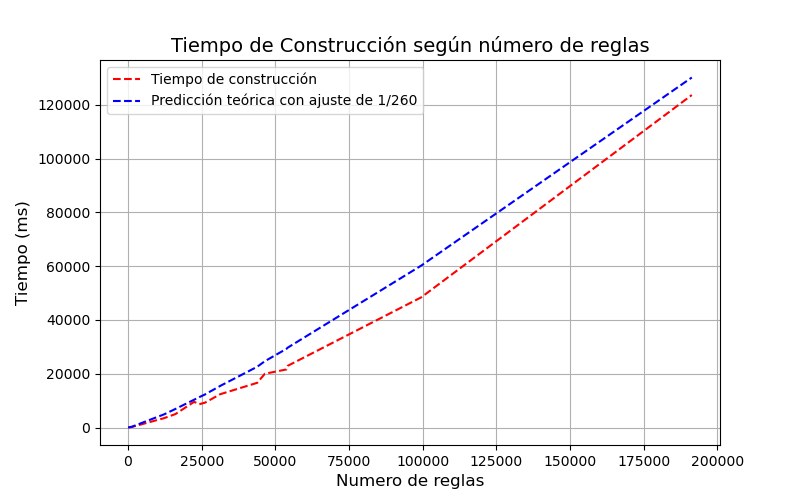
\includegraphics[width=1\textwidth]{imagenes/Time_Construction.png} % Adjust width as needed
    \label{fig:timecst}
\end{figure}

La implementación demuestra comportarse exactamente como lo predicho por la fórmula obtenida del análisis teórico.

ES posible, con memoización, reducir el tiempo de construcción significativamente. Como las primeras reglas corresponden a las reglas creadas por \textit{Re-Pair}, estas se expanden primero y se guardan. Luego, el resto de las reglas corresponden a las reglas extras creadas para reducir la secuencia \textit{C}, y por lo tanto utilizan todas la memoización de forma consecutiva. Sin embargo, esta técnica utiliza significativa memora extra, y no logra comprimir el texto. 



\subsubsection{Búsqueda}


El costo de tiempo teórico para reportar \textit{occ} ocurrencias de un patrón \textit{P} de largo \textit{m} en el texto \textit{T} de largo \textit{n} es:
\[
\mathcal{O}( (m + \log{n}) m \log{r} \log{\log{r}} + \textit{occ} \log{n} \log{\log{r}}  )
\]

Esto se debe a que en una gramática balanceada, el árbol sintáctico tiene altura $\log{n}$, y la operación de acceso en la secuencia representada por permutaciones (\textit{R}) tiene un tiempo $\mathcal{O}(\log \log r)$. De aquí que el primer sumando en la expresión teórica corresponde a expandir \textit{m} símbolos de una regla ($(m + \log{n}) \log{\log{r}}$), por cada comparación en la búsqueda binaria ($\log{r}$), por cada división de sufijo y prefijo del patrón (\textit{m}). El segundo sumando en tanto corresponde a recorrer virtualmente hasta la raíz el árbol sintáctico ($\log{n}$), por cada ocurrencia encontrada (\textit{occ}), haciendo accesos en \textit{R} ($\log{\log{r}}$).

Para medir el tiempo de búsqueda de la implementación en función de los parámetros, se crearon textos que permitiesen mantener fijos algunos de estos y variar el parámetro relevante. Por ejemplo, dado un texto $T = (a^{i}b)^j$ con $i \geq 0$ y $j > 0$, las búsquedas para cualquier patrón $P = a^{k}b$ con $0 \leq k \leq i$ reportan siempre \textit{j} ocurrencias. Con esto se puede medir como varía el tiempo en función del largo de \textit{P}. La figura \ref{fig:timepl} muestra las mediciones de tiempo para la búsqueda de un patrón $a^{k}b \backslash n$ en el texto donde ese patrón entrega la misma cantidad de ocurrencias, independiente del valor de \textit{k}.

\begin{figure}[h!]
    \centering
    \captionsetup{position=above} % Places the caption above the image
    \caption{Tiempo de búsqueda en función del largo del patrón para un mismo número de ocurrencias}
    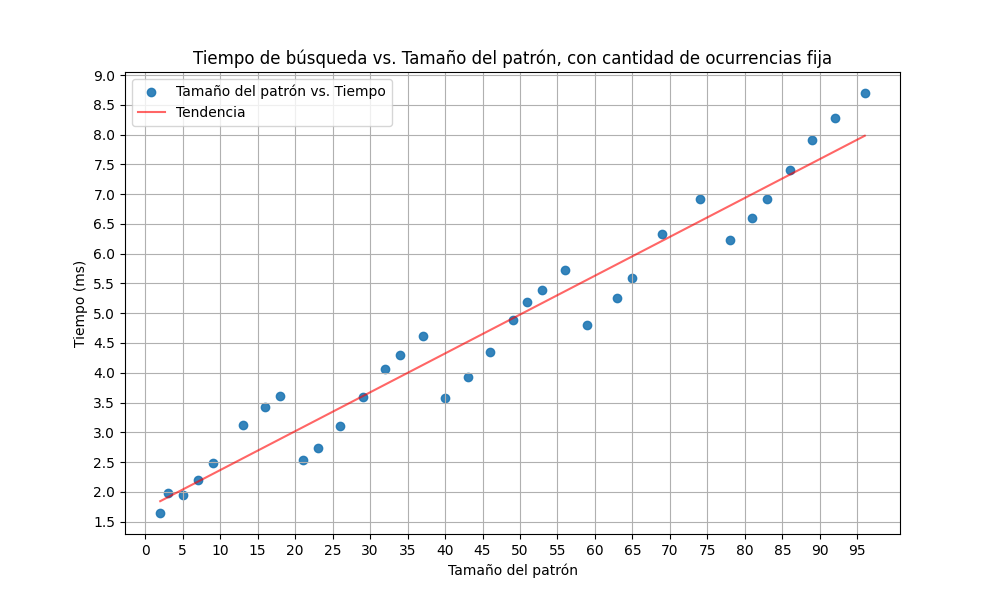
\includegraphics[width=1\textwidth]{imagenes/TIME_FIXED_OCC.png} % Adjust width as needed
    \label{fig:timepl}
\end{figure}

La implementación demuestra un rendimiento equivalente al análisis teórico de la función de búsqueda.

El tiempo en función de la cantidad de ocurrencias requiere mantener fijo el largo de los patrones de búsqueda (además de los otros parámetros). Una solución simple fue usar los bigramas (secuencias de largo 2) más comunes en Inglés\cite{bigram} como los patrones a buscar. Luego se buscan las ocurrencias de estos patrones en varios textos en inglés. Los gráfico de estas medición para cada texto real utilizado correspondes a la figuras de la tablas \ref{tab:searches} y \ref{tab:searchescont}. El gráfico \ref{fig:timeoccs} muestra la combinación de todas las mediciones y la tendencia combinada polinomial de primer grado. 

La figura \ref{fig:timeoccsprediction} ilustra el tiempo teórico para fines de cerciorar el mismo crecimiento, utilizando valores promedios de \textit{n} y \textit{r}. La justificación para esto es que, aunque el tiempo de búsqueda es función de \textit{n} y \textit{r}, además de \textit{occ}, es posible un análisis más simple considerando \textit{r} y \textit{n} como funciones lineales de \textit{occ} en textos reales, donde independiente del largo el texto no se vuelve menos o más predictivo, y la "densidad" de ocurrencias se mantiene igual. 

\begin{figure}[h!]
    \centering
    \captionsetup{position=above} % Places the caption above the image
    \caption{Tiempo de búsqueda en función del número de ocurrencias para un patrón de largo dos}
    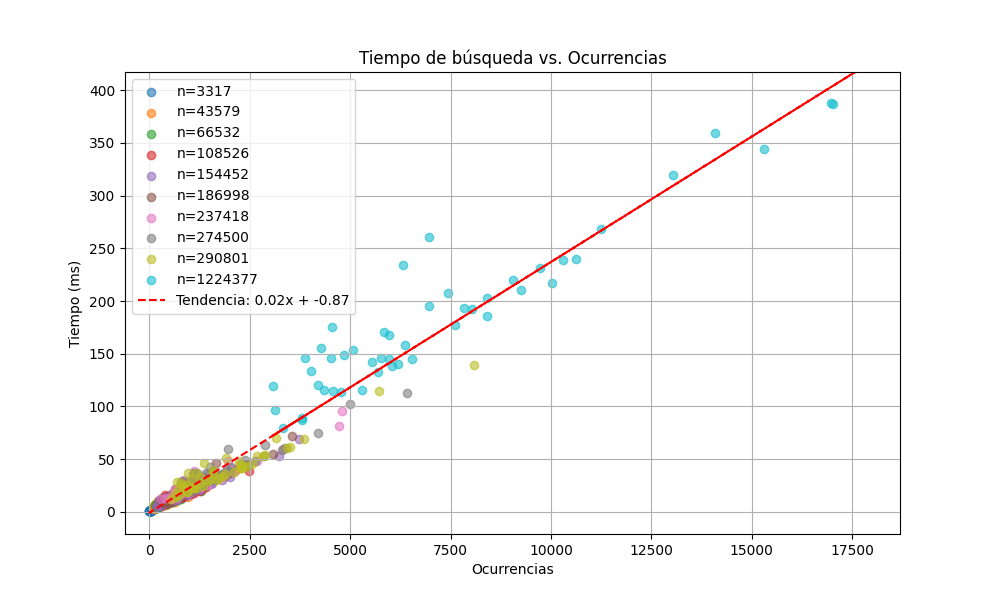
\includegraphics[width=1\textwidth]{imagenes/Time_Fixed_Pattern.png} % Adjust width as needed
    \label{fig:timeoccs}
\end{figure}

\begin{figure}[h!]
    \centering
    \captionsetup{position=above} % Places the caption above the image
    \caption{Tiempo de búsqueda en función del número de ocurrencias para un patrón de largo dos con predicción teórica usando promedio de \textit{n} y \textit{r}, con tiempo teórico 
    $ O( (m + \log{n}) m \log{r} \log {\log {r}} + occ \log{n} \log {r} ) $.}
    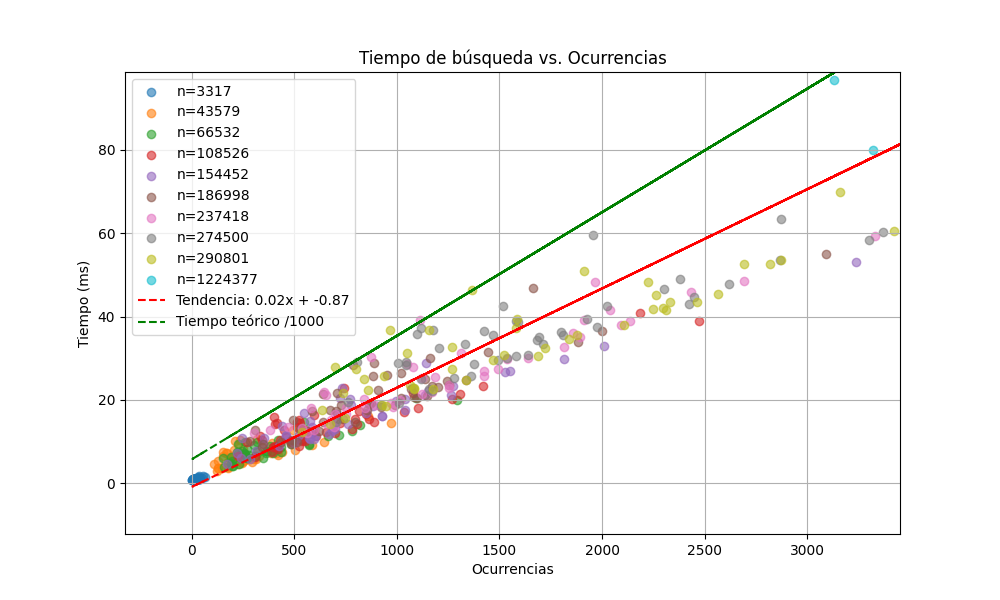
\includegraphics[width=1\textwidth]{imagenes/TIME_SEARCH_ZOOM.png} % Adjust width as needed
    \label{fig:timeoccsprediction}
\end{figure}

\begin{figure}[]
    \centering
    \captionsetup{position=above}
    \caption{Tiempos de búsquedas en \textit{ms} (milisegundos) en función del número de ocurrencias para un patrón de largo 2}
    \hspace*{-\marginparwidth}
    \begin{tabular}{cc} % Two columns      
        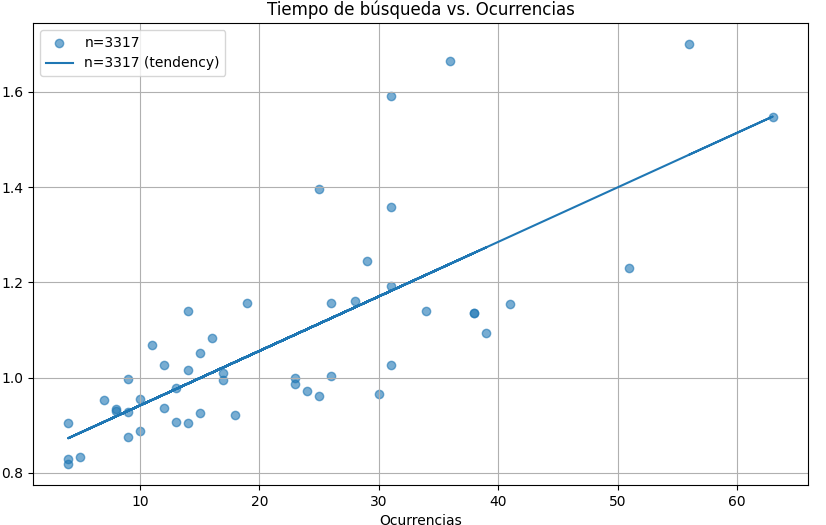
\includegraphics[width=0.55\textwidth]{imagenes/Figure_3317.png} & 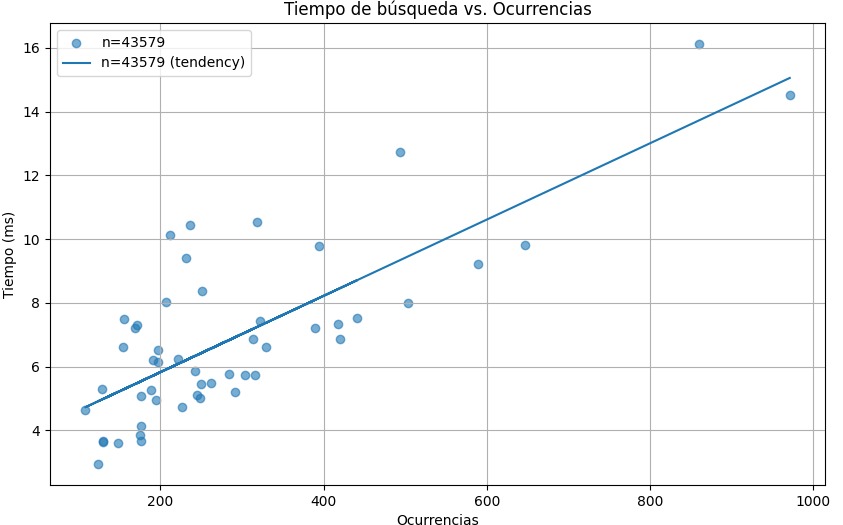
\includegraphics[width=0.55\textwidth]{imagenes/Figure_43579.png} \\
        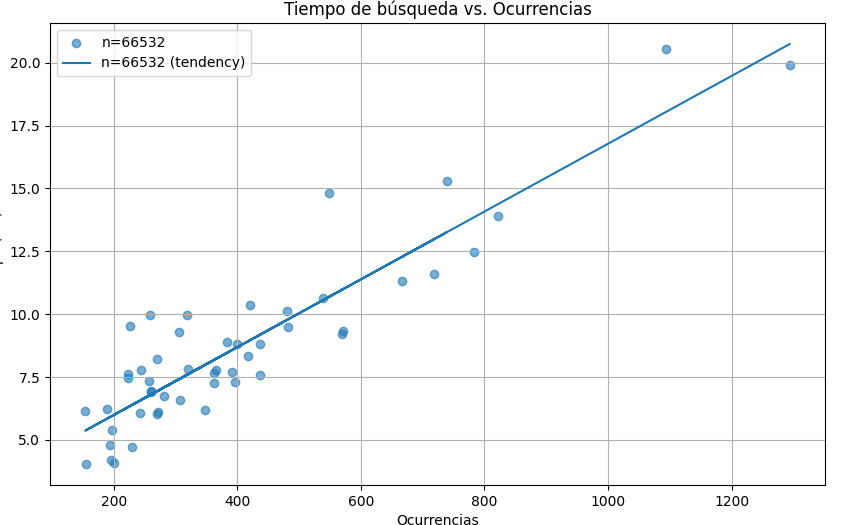
\includegraphics[width=0.55\textwidth]{imagenes/Figure_66532.png} & 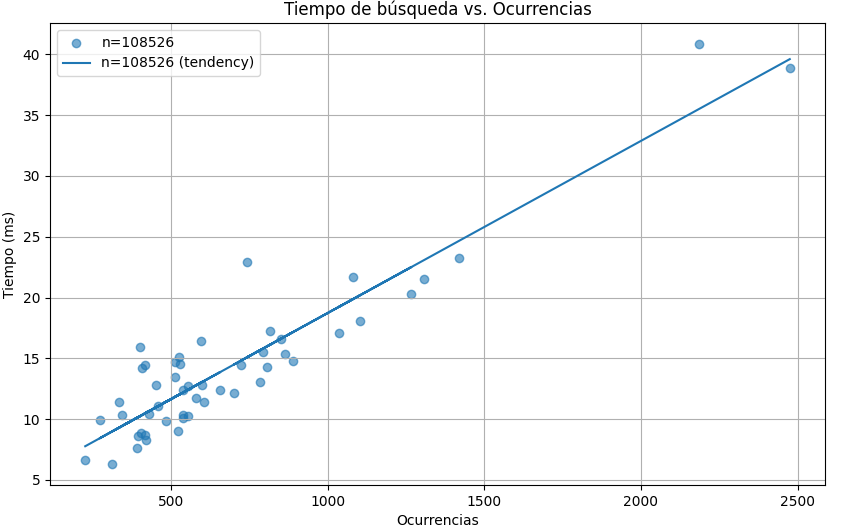
\includegraphics[width=0.55\textwidth]{imagenes/Figure_108526.png} \\
        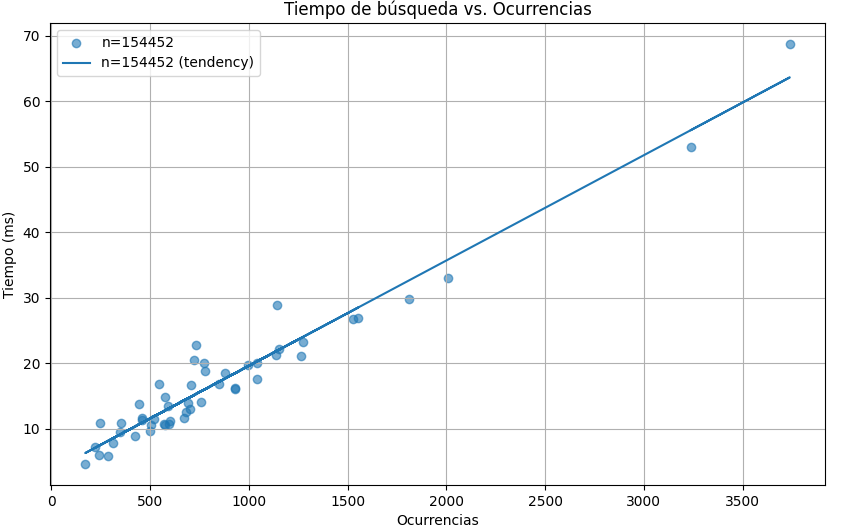
\includegraphics[width=0.55\textwidth]{imagenes/Figure_154452.png} & 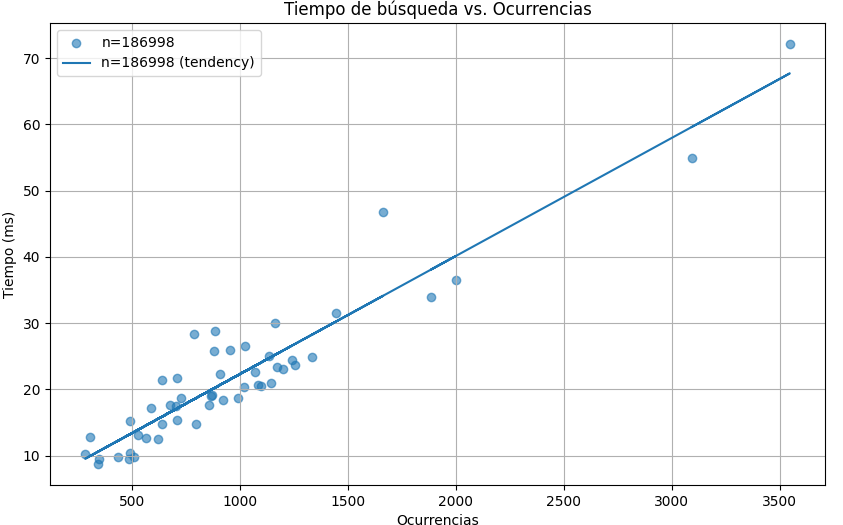
\includegraphics[width=0.55\textwidth]{imagenes/Figure_186998.png} \\
        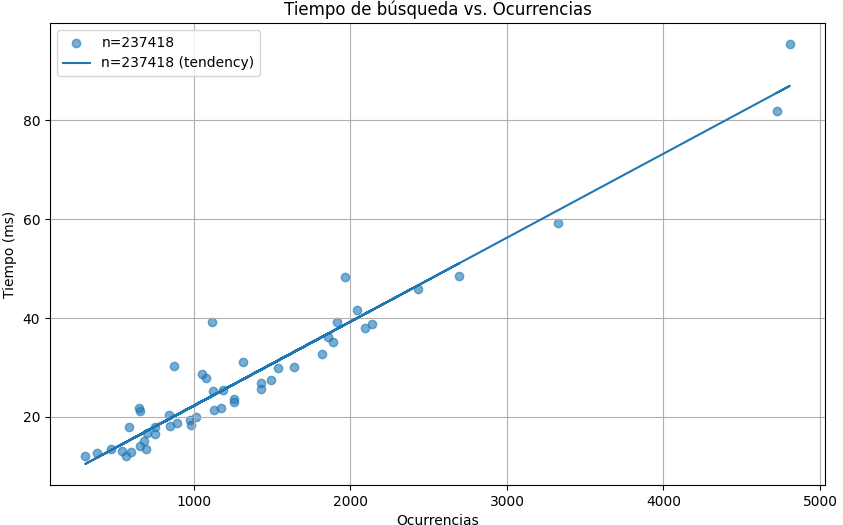
\includegraphics[width=0.55\textwidth]{imagenes/Figure_237418.png} & 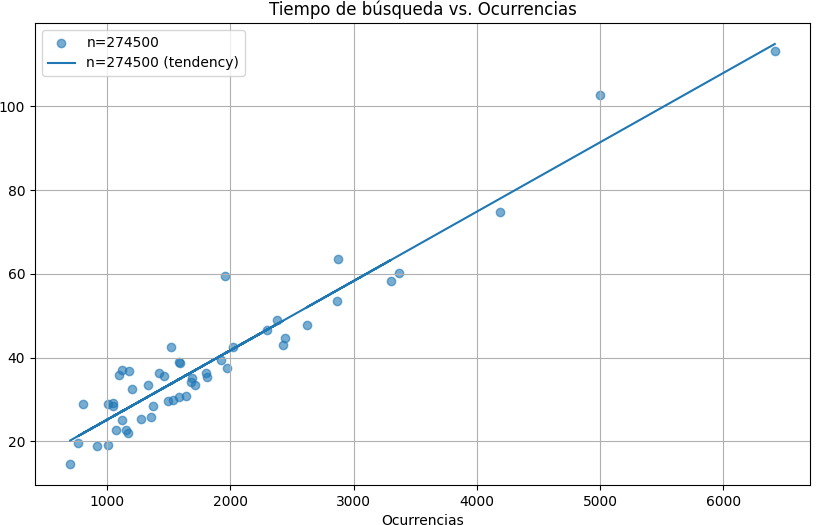
\includegraphics[width=0.55\textwidth]{imagenes/Figure_274500.png} \\
    \end{tabular}    
    \label{tab:searches}
\end{figure}

\begin{figure}[]
    \centering
    \captionsetup{position=above}
    \caption{Tiempos de búsquedas en \textit{ms} (milisegundos) en función del número de ocurrencias para un patrón de largo 2 (Continuación)}
    \hspace*{-\marginparwidth}
    \begin{tabular}{cc} % Two columns      
        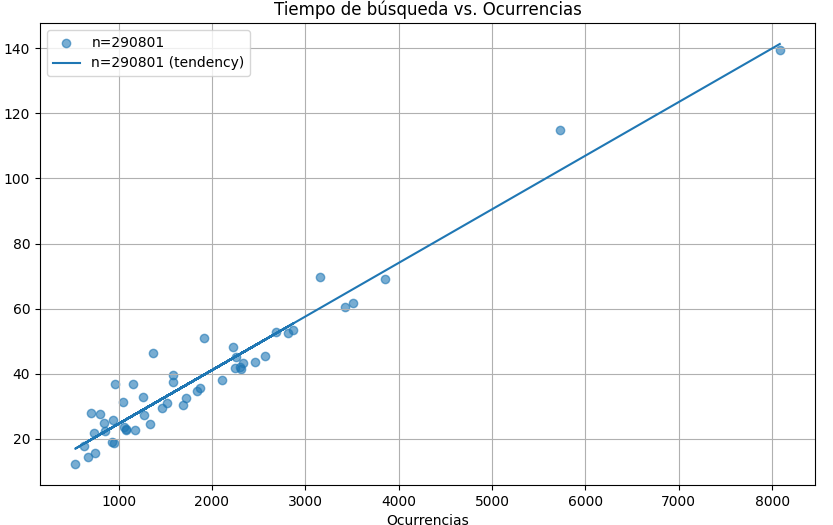
\includegraphics[width=0.55\textwidth]{imagenes/Figure_290801.png} & 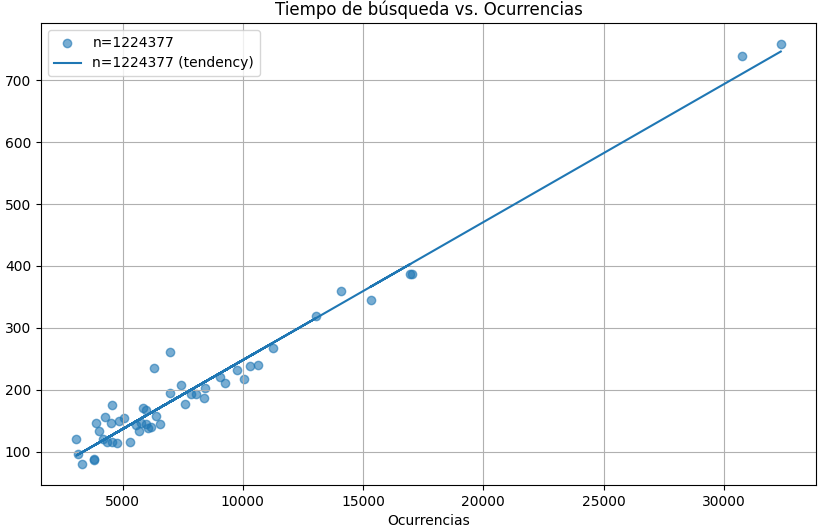
\includegraphics[width=0.55\textwidth]{imagenes/Figure_1224377.png} \\
    \end{tabular}    
    \label{tab:searchescont}
\end{figure}



El tiempo de búsqueda corresponde a la suma de los tiempos de búsqueda binaria de rangos en la grilla, el costo temporal de reportar las reglas dentro de estos rangos y los tiempos de búsqueda de ocurrencias para cada regla reportada. 

La búsqueda binaria demora en el peor caso $m\log{c}$, pues la comparación puede requerir expandir la regla entera hasta el largo del patrón (\textit{m}), y la regla puede corresponder a la regla inicial que expande al texto inicial de largo \textit{n}. En la práctica, con un texto real, la gran mayoría de las comparaciones terminan en el primer símbolo de la expansión. Esto es fácil de ver: como la distribución de los primeros símbolos de las expansiones de las reglas es aproximadamente uniforme (en realidad, es la distribución según las frecuencias de los símbolos en el lenguaje específico) las comparaciones perezosas retornarán falso en el primer símbolo. 

En un texto altamente repetitivo, las expansiones serán más largas, sin embargo, la cantidad de reglas es mucho menor que la de un texto real. Esto significa que no sólo la búsqueda binaria se hace sobre un espacio menor, el reporte de ocurrencias se hace sobre un árbol más corto (si se considera la búsqueda de ocurrencias como el recorrido del árbol sintáctico hasta la raíz).

Las pruebas de medición de tiempo muestran resultados consistentes a lo esperado en todos los casos, por lo cual se puede concluir que la implementación es correcta. 

\newpage
\section{Análisis en textos altamente repetitivos}
\label{sect:repet}

Las colecciones de textos reales altamente repetitivos de \textit{Pizza \& Chili Corpus}\cite{pizzachili_repcorpus} sirven como entradas para pruebas del mismo tipo a las utilizadas por el índice comprimido basado en gramática\cite{claude2020} y son por lo tanto una buena forma de analizar la competitividad de la estructura utilizada. El tamaño de los textos varía desde 45 MiB (\textit{world\_leaders}) a 446 MiB (\textit{einstein.en}), con variados grados de repetición, como se ve en la tabla \ref{tab:collect}. En la misma tabla aparece el espacio de la estructura para cada set de datos como \textbf{\textit{bps}} (bits por símbolo). 

\iffalse
\begin{table}[h!]
\centering
\begin{tabular}{|l|c|c|c|c|}
\hline
\textbf{Colección} & \textbf{Largo} & \textbf{Reglas} & \textit{bps} (estimación) & \textit{bps} (real) \\ \hline  
world\_leaders & 46968181 & 307066 &  0.649 & 8.224 \\ \hline  
Escherichia\_Coli & 112689515 & 3619577 &  3.629 & 40.560\\ \hline  
influenza & 154808555 &1557878 &  1.098 & 12.757 \\ \hline  
kernel & 257961616 &1129349 &  0.474 & 5.532 \\ \hline  
coreutils & 205281778 & 1994376 & 1.077 & 12.270\\ \hline
para&429265758 &4222046 &  1.138 & 12.463 \\ \hline  
cere & 461286644 & 3212008 & 0.796 & 8.809 \\ \hline
einstein.en & 467626544  & 163417 &  0.034 & 0.441 \\ \hline  
\end{tabular}
\caption{Propiedades de cada colección}
\label{tab:collect-old}
\end{table}
Nótese que la medida real de \textit{bps} es mucho más alta que la estimada y eso se debe a la forma en que están implementados los vectores de bits de la librería \textit{SDSL}\cite{sdsl-lite}: estos vectores de bits que corresponden a los pedazos de la secuencia representada por permutaciones no son buenos para tamaños muy pequeños, ya que la cantidad de memoria usada por los metadatos de la implementación del vector son del orden de los 136 Bytes (1088 bits). Por consiguiente, teniendo en cuenta que estos vectores se crean en proporción al alfabeto de tamaño \textit{r}, y la gran mayoría de estos vectores de bits tienen largo 2 bits (de hecho, todos los que corresponden a las reglas extras generadas en \ref{sect:extrar}), sumado a esto la misma magnitud de bits para soportar \textit{rank} y \textit{select}, el tamaño total empírico de los vectores en la secuencia representada por permutaciones es ordenes mayores a lo estimado (para las colecciones medidas, los \textit{bps} reales son 10 veces más grande a los esperado). Una solución a este problema se discute en la sección \ref{section:medic}.
\fi

\begin{table}[h!]
\centering
\begin{tabular}{|l|c|c|c|c|}
\hline
\textbf{Colección} & \textbf{Largo} & \textbf{Reglas} & \textit{bps}\\ \hline  
world\_leaders & 46968181 & 307066 &  0.848511 \\ \hline  
Escherichia\_Coli & 112689515 & 3619577 &  4.55733 \\ \hline  
influenza & 154808555 &1557878 & 1.40496\\ \hline  
kernel & 257961616 &1129349 & 0.619162 \\ \hline  
coreutils & 205281778 & 1994376 & 1.36035 \\ \hline
para&429265758 &4222046 &  1.41742 \\ \hline  
cere & 461286644 & 3212008 & 0.986939 \\ \hline
einstein.en & 467626544  & 163417 &  0.0475765 \\ \hline  
\end{tabular}
\caption{Propiedades de cada colección}
\label{tab:collect}
\end{table}



Para cada colección se hicieron búsquedas de patrones aleatorios de ciertos largos y se midieron los tiempos de búsqueda por ocurrencia. La figura \ref{fig:searchpizza} muestra los resultados obtenidos, ilustrados en un gráfico donde las escalas de ambos ejes son logarítmicas, y el eje \textit{Y} corresponde a los tiempos por ocurrencia (en teoría, $\mathcal{O}( (m + \log{n}) m \log{r} \log{\log{r}} + \textit{occ} \log{n} \log{\log{r}}) / \textit{occ}$), mientras que el eje \textit{X} corresponde a la cantidad \textit{occ} de ocurrencias detectadas.  

\begin{figure}
    \centering
    \captionsetup{position=above}
    \caption{Tiempos por ocurrencia en $\mu s$ (microsegundos) de búsquedas en función del número de ocurrencias para distintas colecciones repetitivas. Ambos ejes están es escala logarítmica}
    \hspace*{-\marginparwidth}
    \begin{tabular}{cc} % Two columns      
        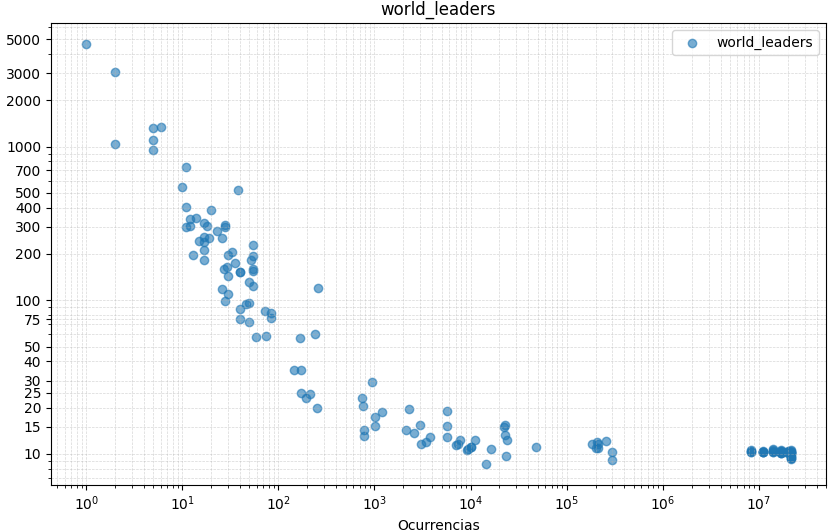
\includegraphics[width=0.55\textwidth]{imagenes/SEARCH_world_leaders.png} & 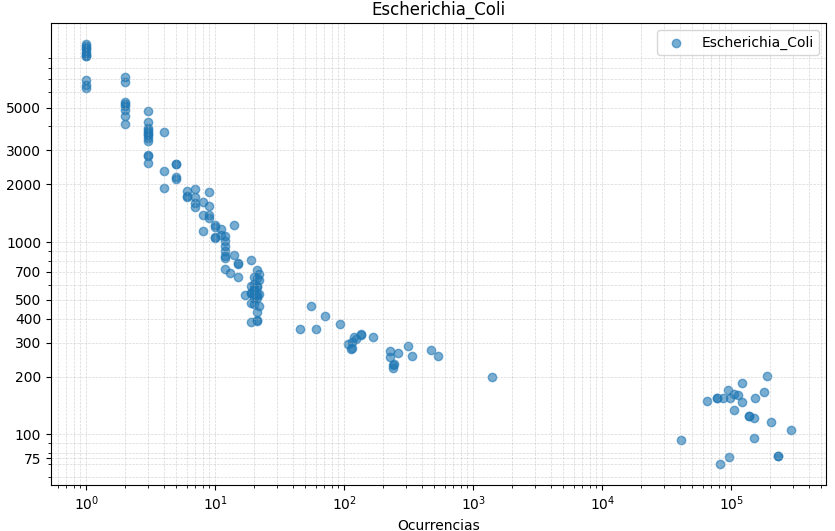
\includegraphics[width=0.55\textwidth]{imagenes/SEARCH_Escherichia.png} \\
        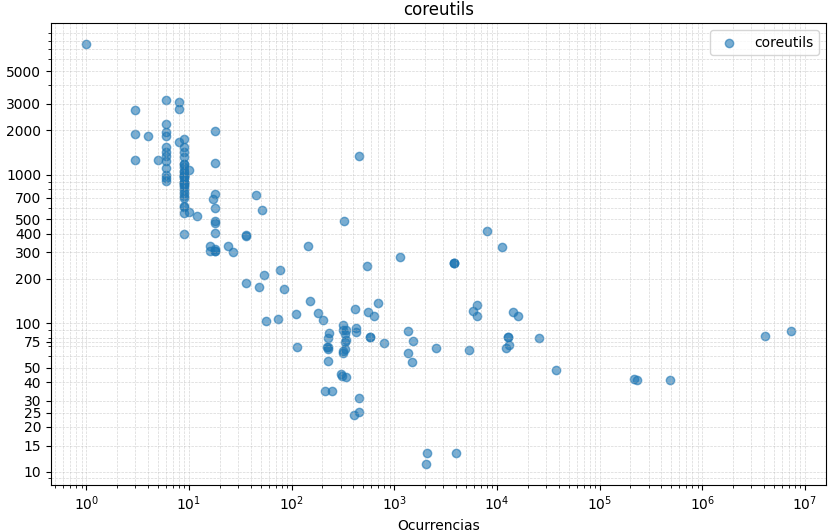
\includegraphics[width=0.55\textwidth]{imagenes/SEARCH_coreutils.png} & 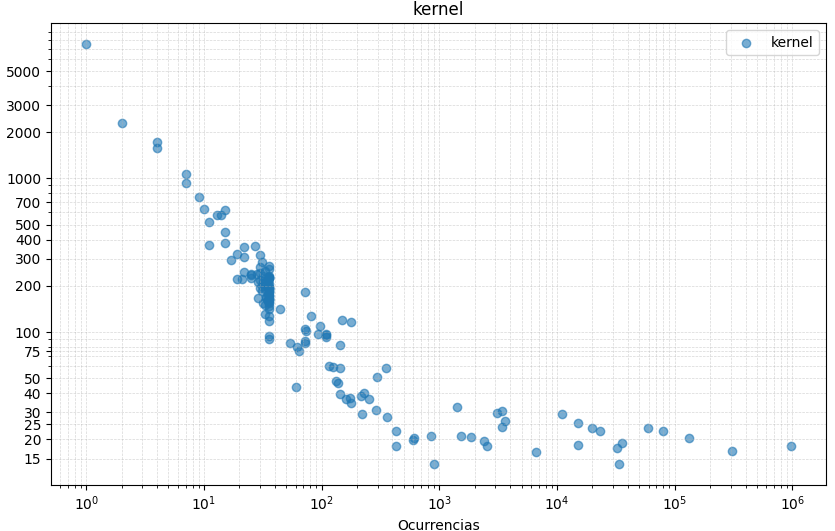
\includegraphics[width=0.55\textwidth]{imagenes/SEARCH_kernel.png} \\
        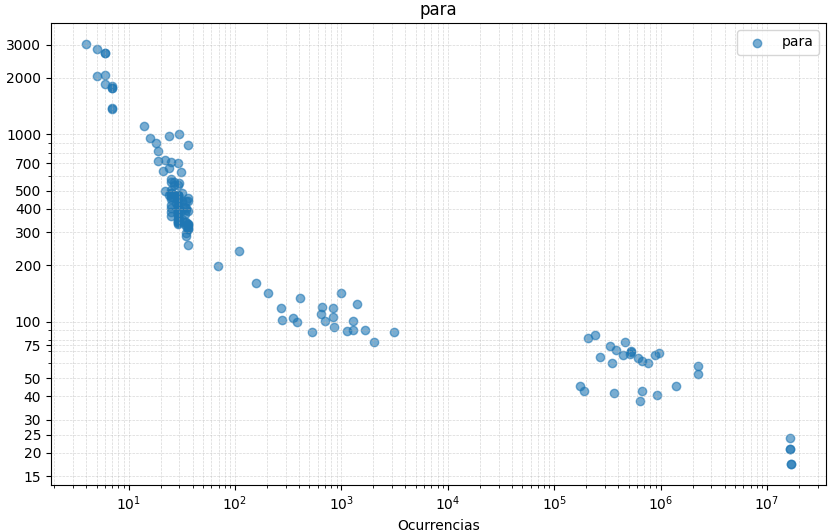
\includegraphics[width=0.55\textwidth]{imagenes/SEARCH_para.png} & 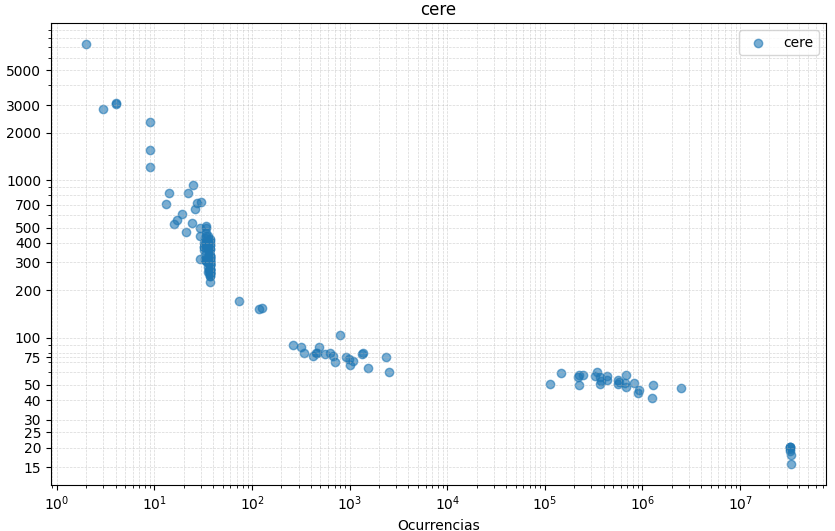
\includegraphics[width=0.55\textwidth]{imagenes/SEARCH_cere.png} \\
        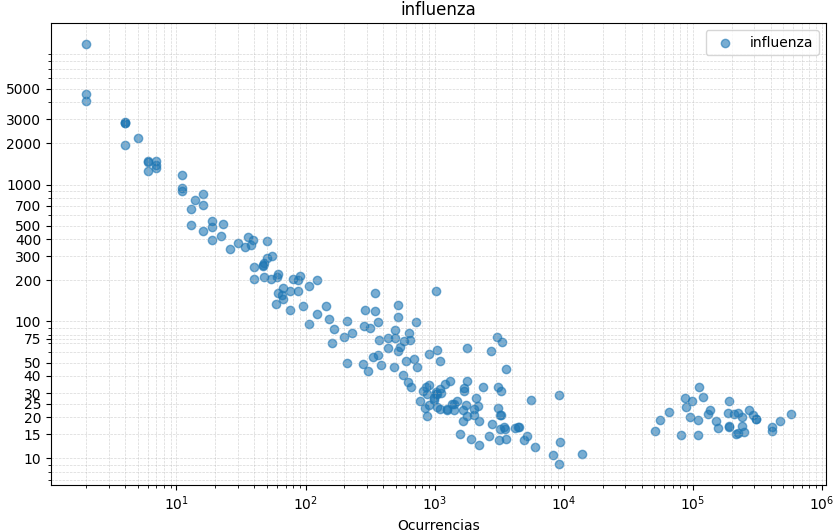
\includegraphics[width=0.55\textwidth]{imagenes/SEARCH_influenza.png} & 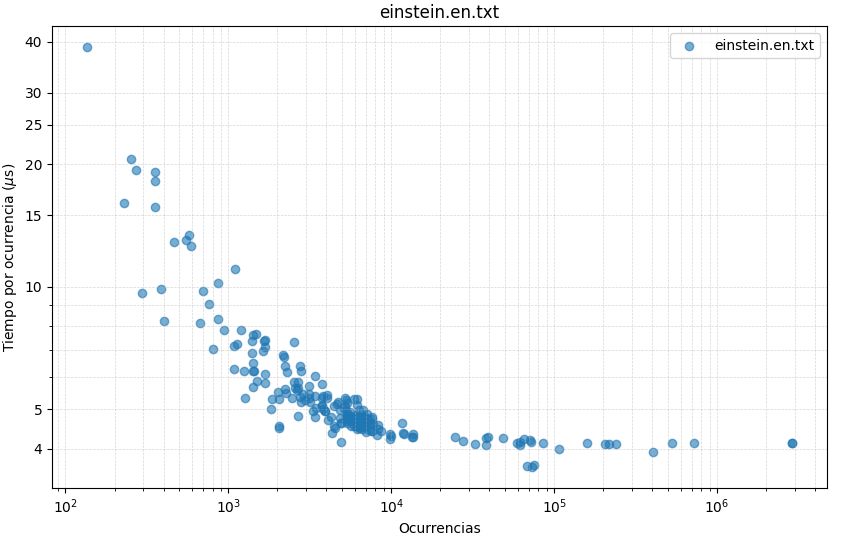
\includegraphics[width=0.55\textwidth]{imagenes/SEARCH_einstein.png} \\
    \end{tabular}    
    \label{fig:searchpizza}
\end{figure}

La estructura toma tiempos menores por ocurrencia mientras más ocurrencias del patrón se encuentren en el texto. Patrones de menos largo aparecen con más incidencia en los textos y por lo tanto el proceso de dividir el patrón en todos sus posible sufijos y prefijos es más corto. 

En colecciones altamente repetitivas como \textit{einstein.en} logra tiempos de búsqueda por ocurrencia bajo 5 $\mu s$ cuando la cantidad de ocurrencias es del orden de $10^4$ o mayor. En \textit{world\_leaders} el tiempo por ocurrencia se estabiliza en 9 a 10 $\mu s$. En otras colecciones el tiempo por ocurrencia es menos estable: en \textit{influenza} altas ocurrencias tienen tiempo por ocurrencia entre 5 a 30 $\mu s$.

Se analizó el caso para patrones aleatorios de largo fijo $m = 10$ sobre la colección \textit{einstein.en}. Los resultados se muestran en la figura \ref{fig:searcheinsteinm10} donde la búsqueda alcanza tiempos estables de 5 $\mu s$ por ocurrencia para patrones con ocurrencias superiores a $10^3$.

\begin{figure}
    \centering
    \captionsetup{position=above}
    \caption{Tiempos por ocurrencia en $\mu s$ (microsegundos) de búsquedas de patrones aleatorios de largo fijo 10 en función del número de ocurrencias en la colección \textit{einstein.en}. El eje X está en escala logarítmica}
    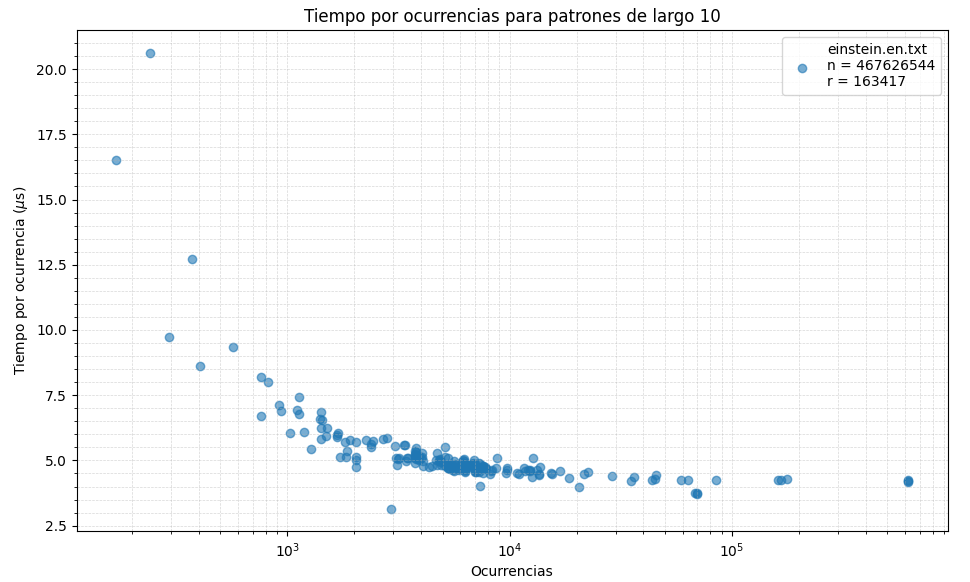
\includegraphics[width=1\textwidth]{imagenes/TIME_M10_EINSTEIN.png} 
    \label{fig:searcheinsteinm10}
\end{figure}

\section{Análisis comparativo con la solución lineal de búsqueda sin compresión}

El reporte de ocurrencia de patrones utilizando un algoritmo lineal en un texto sin comprimir tiene un tiempo de búsqueda en el peor caso de $\mathcal{O}(n m)$, con \textit{n} el largo del texto y \textit{m} el largo del patrón. En un texto real sin embargo, el tiempo es más cercano a $\mathcal{O}(n)$, pues la gran mayoría de las comparaciones terminan en el primer símbolo, es decir, el tiempo es relativamente independiente al largo del patrón.


\begin{table}[h!]
\centering
\begin{tabular}{|l|l|c|c|c|c|c|}
\hline
\textbf{n} & \textbf{r} & \textbf{m} & \textbf{occ} & \textbf{t(ms) estructura} & t(ms) lineal & t(ms) teórico \\ \hline
111299 & 26149 & 5 & 14 & \textbf{4.34} & 10.85 & 10.08 \\
111299 & 26149 & 10 & 1 & \textbf{4.36} & 10.76 & 10.17 \\
111299 & 26149 & 20 & 1 & \textbf{5.41} & 15.76 & 10.49 \\
111299 & 26149 & 30 & 1 & \textbf{6.14} & 15.74 & 10.98 \\
111299 & 26149 & 40 & 1 & \textbf{7.11} & 15.77 & 11.61 \\
111299 & 26149 & 50 & 1 & \textbf{7.85} & 15.88 & 12.41 \\
111299 & 26149 & 70 & 1 & \textbf{9.81} & 16.16 & 14.46 \\
111299 & 26149 & 100 & 1 & \textbf{11.72 }& 15.72 & 18.72 \\ \hline
290801 & 54170 & 5 & 93 & \textbf{7.88} & 28.77 & 10.17 \\
290801 & 54170 & 10 & 3 &\textbf{ 6.37 }& 28.68 & 10.20 \\
290801 & 54170 & 20 & 1 & \textbf{7.18} & 42.79 & 10.56 \\
290801 & 54170 & 30 & 1 & \textbf{8.15 }& 41.55 & 11.10 \\
290801 & 54170 & 40 & 1 & \textbf{9.24} & 42.41 & 11.81 \\
290801 & 54170 & 50 & 1 & \textbf{10.25} & 42.17 & 12.70 \\
290801 & 54170 & 70 & 1 & \textbf{12.41} & 41.76 & 14.98 \\
290801 & 54170 & 100 & 1 & \textbf{15.33} & 41.75 & 19.71 \\ \hline
704731 & 119734 & 5 & 640 & \textbf{21.11 }& 69.06 & 10.79 \\
704731 & 119734 & 10 & 216 & \textbf{12.15 }& 68.66 & 10.46 \\
704731 & 119734 & 20 & 75 & \textbf{10.71 }& 99.65 & 10.72 \\
704731 & 119734 & 30 & 1 & \textbf{ 9.41} & 99.67 & 11.24 \\
704731 & 119734 & 40 & 1 & \textbf{10.68} & 99.75 & 12.04 \\
704731 & 119734 & 50 & 1 & \textbf{11.78} & 99.69 & 13.02 \\
704731 & 119734 & 70 & 1 & \textbf{13.63} & 99.64 & 15.56 \\
704731 & 119734 & 100 & 1 & \textbf{16.94} & 99.26 & 20.80 \\ \hline
1224377 & 191364 & 5 & 329 & \textbf{17.24 }& 118.98 & 10.48 \\
1224377 & 191364 & 10 & 10 & \textbf{9.06} & 118.91 & 10.25 \\
1224377 & 191364 & 20 & 1 & \textbf{9.48} & 172.84 & 10.69 \\
1224377 & 191364 & 30 & 1 & \textbf{10.55} & 172.58 & 11.33 \\
1224377 & 191364 & 40 & 1 & \textbf{11.90} & 173.20 & 12.18 \\
1224377 & 191364 & 50 & 1 & \textbf{13.23} & 173.08 & 13.22 \\
1224377 & 191364 & 70 & 1 & \textbf{16.16} & 172.97 & 15.92 \\
1224377 & 191364 & 100 & 1 & \textbf{19.24} & 172.31 & 21.47 \\ \hline
2205984 & 333238 & 5 & 409 & \textbf{31.03} & 221.59 & 10.61 \\
2205984 & 333238 & 10 & 11 & \textbf{10.39} & 222.08 & 10.28 \\
2205984 & 333238 & 20 & 1 & \textbf{11.35} & 327.83 & 10.74 \\
2205984 & 333238 & 30 & 1 & \textbf{11.98 }& 320.78 & 11.43 \\
2205984 & 333238 & 40 & 1 & \textbf{13.65 }& 323.65 & 12.34 \\
2205984 & 333238 & 50 & 1 & \textbf{14.92} & 323.42 & 13.46 \\
2205984 & 333238 & 70 & 1 & \textbf{17.48} & 317.41 & 16.34 \\
2205984 & 333238 & 100 & 1 & \textbf{22.68} & 326.57 & 22.27 \\ \hline

\end{tabular}
\caption{Tiempos de búsqueda en textos reales de largo \textit{n} de patrones aleatorios de largo \textit{m}, con \textit{occ} ocurrencias en promedio y con \textit{r} la cantidad de reglas}
\label{tab:runtimes}
\end{table}

El costo temporal teórico de la estructura en reportar $occ$ ocurrencias, considerando $r$ como el número de reglas al comprimir el texto por gramática es:
\[
\mathcal{O}( (m + \log{n}) m \log{r} \log{\log{r}} + \textit{occ} \log{n} \log{\log{r}}  )
\]
Para que lo anterior sea menor al tiempo de búsqueda lineal, con un patrón de largo $m < \log {n}$ se debe cumplir que:
\[occ = o ( \frac{n}{ \log n \log \log r} ) \]

Los valores de \textit{occ} y \textit{r} serán pequeños si el texto es repetitivo y las ocurrencias del patrón de búsqueda son pocas. Este es el caso para textos reales como se aprecia en la tabla \ref{tab:runtimes}. Con largos de patrones suficientemente largos, las ocurrencias en textos reales tienden a ser únicas. La naturaleza de los textos reales hace que la "densidad" de repetitividad sea relativamente constante, y por lo tanto, la cantidad de ocurrencias de patrones crece más lento que el largo del texto. Esto implica que el algoritmo termina venciendo con más holgura a la búsqueda lineal mientras más largo sea el texto, al menos en el contexto de textos reales como lo son las novelas, los ensayos, \textit{etc}.

Con \textit{r} pequeño la grilla es pequeña y por lo tanto las búsquedas de rango son más cortas, además el árbol sintáctico es más pequeño y por lo tanto las búsquedas de ocurrencias hasta la raíz son más cortas. Con \textit{occ} pequeño la cantidad de búsquedas de ocurrencias son menores. Las ocurrencias \textit{occ} suelen ser proporcionales, tomando patrones aleatorios de un largo fijo, a qué tan repetitivo es el texto, es decir, en general, $occ \propto r ^{-1}$.

Para ejemplificar lo anterior, considere el siguiente texto $T$: 

\verb|"aaaaaaaaaabaaaaaaaaaab...aaaaaaaaaab\n..."|

Esto es, un texto de muchas líneas donde cada línea corresponde a la repetición de un patrón de cierta cantidad de \textit{a} seguidas de una \textit{b}. El texto es muy repetitivo, como se aprecia en la tabla \ref{tab:runtimes2} por la pequeña cantidad de reglas, y si se buscan patrones de la forma $a^{i}b$\verb|\n| que son los más raros, el buscador de la estructura es más rápido que la búsqueda lineal:

\begin{table}[h!]
\centering
\begin{tabular}{|l|l|c|c|c|c|c|}
\hline
\textbf{n} & \textbf{r} & \textbf{m} & \textbf{occ} & \textbf{t(ms) estructura} & t(ms) lineal & t(ms) teórico \\ \hline
69120 & 22 & 5 & 720 & 1.89 & 6.80 & 10.31 \\
69120 & 22 & 10 & 720 & 2.59 & 6.85 & 10.32 \\
69120 & 22 & 20 & 720 & 3.73 & 10.12 & 10.37 \\
69120 & 22 & 30 & 720 & 3.65 & 9.97 & 10.44 \\
69120 & 22 & 40 & 720 & 3.45 & 9.85 & 10.54 \\
69120 & 22 & 50 & 720 & 4.90 & 9.83 & 10.65 \\
69120 & 22 & 70 & 720 & 6.25 & 9.91 & 10.96 \\  \hline

\end{tabular}
\caption{Tiempos de búsqueda en texto repetitivo con \textit{n} el largo del texto original, \textit{r} la cantidad de reglas, \textit{m} el largo del patrón. }
\label{tab:runtimes2}
\end{table}

Considérese un ejemplo más realista. Se tiene una secuencia de ADN como un texto donde el alfabeto es $A, T, G, C$. Estas secuencias son sumamente largas, y buscar una cadena específica en esta usando una búsqueda lineal puede ser muy lento, en especial si se requiere repetir el proceso varias veces con distintos patrones de pocas ocurrencias. En este caso, la estructura tiene un tiempo de búsqueda más corto que la búsqueda lineal, como se aprecia en la tabla \ref{tab:runtimes3}.

\begin{table}[h!]
\centering
\begin{tabular}{|l|l|c|c|c|c|c|}
\hline
\textbf{n} & \textbf{r} & \textbf{m} & \textbf{occ} & \textbf{t(ms) estructura} & t(ms) lineal & t(ms) teórico \\ \hline  
1000000 & 182668 & 5 & 975 & 83.17 & 98.23 & 11.21 \\
1000000 & 182668 & 10 & 2 & 10.49 & 98.78 & 10.24 \\
1000000 & 182668 & 20 & 1 & 9.79 & 142.39 & 10.68 \\
1000000 & 182668 & 30 & 1 & 11.17 & 142.58 & 11.32 \\
1000000 & 182668 & 40 & 1 & 12.77 & 141.67 & 12.16 \\
1000000 & 182668 & 50 & 1 & 14.05 & 141.11 & 13.19 \\
1000000 & 182668 & 70 & 1 & 16.73 & 140.73 & 15.87 \\
1000000 & 182668 & 100 & 1 & 20.58 & 140.75 & 21.39 \\ \hline
\end{tabular}
\caption{Tiempos de búsqueda en secuencia de ADN de largo 100.000, \textit{occ} es la cantidad de ocurrencias del patrón}
\label{tab:runtimes3}
\end{table}




%\lambda + \lambda \log{r} + r \log{r}    +  2r \log r +       o(r \log r) +       2r \log \sigma
% 16  + 16log16112 + 16112log16112+  2*16112 log 16112 + 16112 log 16112 + 2*16112 log 16112
% 16  + 16 * 14 + 16112*14 +  16112*32 + 16112*14 + 16112*32

\section{Análisis comparativo con índice comprimido basado en gramática}

El índice comprimido basado en gramática\cite{claude2020} es una estructura de datos que permite buscar patrones en un texto comprimido por gramática. La tabla \ref{tab:runtimes4} muestra los tiempos de búsqueda de patrones aleatorios en textos reales con la estructura propuesta en este trabajo y con la estructura del índice comprimido basado en gramática.


\begin{table}[h!]
\centering
\begin{tabular}{|l|l|c|c|c|c|c|}
\hline
\textbf{set} & \textbf{tamaño} & \textbf{m} & \textbf{occ} & \textbf{t(ms) estructura} & t(ms) índice \\ \hline  

\hline
\end{tabular}
\caption{Tiempos de búsqueda para patrones aleatorios de largo \textit{m}, con \textit{occ} ocurrencias}
\label{tab:runtimes4}
\end{table}
% LTeX: language=es-es
\chapter{Conclusiones}
\section{Conclusiones generales}
\subsection{Objetivo general}
Finalizado este trabajo, se puede concluir con suficiente certeza que los objetivos propuestos, esto es, la correcta implementación de la estructura y el análisis empírico de su funcionamiento, fueron completados satisfactoriamente. La estructura se comporta en la práctica como lo teorizado.

En textos reales, la estructura comprimida simplificada para indexar texto basada en gramática logra el reporte de las posiciones de las ocurrencias de patrones de búsqueda en tiempos más cortos que la búsqueda lineal de patrones ($\mathcal{O}( (m + \log{n}) m \log{r} \log{\log{r}} + \textit{occ} \log{n} \log{\log{r}}  )$ versus $\mathcal{O}(n m)$). El espacio usado es de orden similar al texto original, pues a pesar de que se comprime a una cantidad \textit{r} de reglas que es menor al largo \textit{n} del texto, estas reglas requieren más memoria para ser guardadas ($\log r$ bits por cada regla). Sin embargo, textos suficientemente repetitivo logra una compresión significativa, y se benefician de una velocidad de reporte de ocurrencias aún mayor.

En particular, si la cantidad de ocurrencias del patrón es muy pequeña en comparación al tamaño del texto, y el texto en sí es suficientemente repetitivo, la búsqueda es ordenes de magnitud más rápida que una búsqueda lineal. Textos altamente repetitivo son también comprimidos de forma significativa, por ejemplo, los textos correspondientes a las colecciones repetitivas analizados en \ref{sect:repet}

Los tiempos de búsqueda por patrón mejoran enormemente con la cantidad de ocurrencias de un patrón, y esto es consistente con lo esperado. Con respecto al estado del arte, en las colecciones repetitivas evaluadas, los tiempos de búsqueda por ocurrencia son mayores (alrededor de 4 microsegundos más) que los tiempos por ocurrencia de el índice comprimido basado en gramática\cite{claude2020}. Futuras optimizaciones en la implementación podrían mejorar este aspecto y equiparar los tiempos de búsqueda de la estructura.

\section{Cumplimiento de objetivos específicos}
\begin{enumerate}
    \item Implementación la estructura de forma correcta: La implementación de la estructura fue realizada de forma correcta, y se logró una implementación funcional de la estructura propuesta en el libro \textit{Compact Data Structures}.
    \item Implementación de pruebas de robustez y consistencia de la estructura: Se implementaron pruebas de robustez y consistencia de la estructura, las cuales permitieron validar su correcto funcionamiento y su congruencia con el análisis teórico.
    \item Implementación de pruebas de desempeño espacial y temporal de la implementación: Se realizaron pruebas de desempeño espacial y temporal de la implementación, las cuales permitieron evaluar su eficiencia en términos de tiempo y espacio.
    \item Análisis de los resultados de las pruebas para obtener conclusiones respecto al desempeño: Se analizaron los resultados de las pruebas para obtener conclusiones respecto al desempeño empírico de la estructura, identificando sus fortalezas y debilidades.
\end{enumerate}


\iffalse
\section{Medición empírica del espacio de la estructura}
\label{section:medic}

Queda como deuda de este trabajo la medición concreta y empírica del espacio de la estructura en tiempo de ejecución. Para esto es necesario cambiar ciertos elementos de la estructura, en específico, los vectores de bits que representan los pedazos de la secuencia \textit{R} representada por permutaciones. La implementación actual crea $\sigma + r$ vectores de bits, y la gran mayoría de estos tienen tamaño 2 (lo son de esta forma todos los vectores de bits extras creados al expandir las reglas). En teoría esto no es un problema pues los vectores en total suman $2n$ bits de espacio, sin embargo, cada uno de estos tiene un exceso en metadatos de 136 KB. Para solucionar esto basta reemplazar estos vectores por un solo gran vector de bits que corresponde a la concatenación de todos, y utilizar un vector auxiliar para marcar las posiciones de los vectores originales en este vector final. Con esto, se puede hacer una medición empírica más cercana a la estimada en el trabajo en la tabla \ref{tab:collect}.
\fi

\section{Memoizar}

No obstante las virtudes de la estructura, esta requiere un tiempo de construcción no menospreciable. Si se utiliza extra memoria es posible aplicar memoización (regla $\longrightarrow $ expansión) para acelerar el proceso de ordenamiento de las reglas por sus expansiones y así disminuir el tiempo de comparación y por consiguiente construcción, pero esto requiera memoria extra durante el proceso equivalente al mismo texto, es decir, $\mathcal{O}(n \log \sigma)$ bits, con lo cual no hay compresión. 

Se puede limitar la memoización a sólo las reglas originalmente creadas por \textit{Re-Pair} y aprovechar que la estructura del árbol gramatical está balanceada desde el nivel correspondiente a los sub-árboles que salen de tomar pares de símbolos de la secuencia \textit{C}.

Es posible también aplicar memoización en la búsqueda de ocurrencias secundarias, lo cual reduciría enormemente el tiempo de búsqueda de patrones. Esto requeriría memoria de ejecución extra $\mathcal{O}(r \log r)$, pero evitaría re-calcular las ocurrencias de cada regla en el símbolo inicial. Si se considera la búsqueda de ocurrencias como recorrer el árbol sintáctico desde cada nodo equivalente a la regla, este proceso de memoización permite evitar recorrer los mismos nodos más de una vez.

\section{Sobre la secuencia \textit{R}}

La estructura expande la secuencia \textit{R} obtenida de \textit{Re-Pair} con el fin de eliminar la secuencia \textit{C}. Esto implica extender \textit{R} con extras $\mathcal{O}(|C|)$ reglas. Es posible hacer este proceso de extender \textit{R} de una forma puramente virtual, manteniendo \textit{C} y \textit{R} originales. En efecto, el proceso de extender \textit{R} es equivalente a construir un árbol binario con \textit{C} como las hojas del árbol. Con esto, si el programa requiere una regla específica de la secuencia virtual $R'$ como \textit{R} expandida, es fácil saber la posición de esta regla en este árbol virtual, y con eso, se puede saber con exactitud el rango en \textit{C} que corresponde a la regla (si la regla corresponde a las creadas en la expansión). 

La expresión para obtener el rango de \textit{C} que le corresponde a una regla $R_i$ no es simple pero se puede obtener, pues la estructura del árbol virtual es conocida: Las reglas se crean a partir de \textit{C} tomando, en cada iteración, pares de símbolos de izquierda a derecha, reemplazándolos por un nuevo símbolo, dejando símbolos sin par para la siguiente iteración, y así hasta reducir \textit{C} a un solo símbolo. Así, en casos donde el largo de \textit{C} no es una potencia de 2 las posiciones de las reglas son aún calculables.

Cuando la estructura implementada requiera reordenar $R'$ por su expansión izquierda invertida por orden lexicográfico, basta con traducir este reordenamiento a la secuencia $R$ original y \textit{C}.

Lo anterior permite expandir estas reglas extras en tiempo $\mathcal{O}(h_i)$, donde $h_i$ es la altura de la regla en el árbol, lo que implica que expandir todas estas reglas extras, utilizando la técnica descrita, tiene un costo total de tiempo $\mathcal{O}(n)$ y espacio equivalente a la expansión de las reglas originales $\mathcal{O}(n)$. 

Si se añade memoización sobre las reglas originales, expandir cualquier regla extra toma tiempo constante por cada regla que pertenece al rango en \textit{C} correspondiente.

\section{Otras mejoras}

\subsection{Potencial paralelismo}

Es posible también utilizar múltiples \textit{threads} o multihilos en ciertas partes del programa en donde el paralelismo podría mejorar considerablemente la búsqueda, por ejemplo, los dos ordenamientos de las reglas por sus expansiones, las múltiples divisiones del patrón en sus sufijos y prefijos, las cuatro búsquedas binarias para encontrar los rangos de estas divisiones, y las múltiples búsquedas para cada ocurrencia encontrada en la grilla. En teoría, y con suficientes hilos, se puede eliminar el largo del patrón y las ocurrencias. como factores en los tiempos de búsqueda. 


% ver https://www.overleaf.com/learn/latex/Glossaries
% \input{glosario.tex} % opcional

\nocite{*}
\bibliographystyle{plain}
\bibliography{bibliografia}

% opcional ...
\begin{appendices}
\chapter{Anexo}
\begin{lstlisting}[style=cppstyle, caption={Llamando Re-Pair}, label={lst:re-pair-call}]
FILE *input;
DICT *dict;
input  = fopen(input_filename.c_str(), "rb");
dict = RunRepair(input);
fclose(input);
RULE *rules = dict->rule; // set or rules 
CODE *comp_seq = dict->comp_seq; // sequence C
\end{lstlisting}
\begin{lstlisting}[style=cppstyle, caption={Añadir más reglas hasta eliminar C}, label={lst:rule-add}]
while (dict->seq_len > 1) {
    for (u_int i = 0; i < dict->seq_len; i = i+2) {
        if (i == dict->seq_len - 1) { // odd case
            comp_seq[i/2] = comp_seq[i];
        }
        else {
            RULE new_rule;
            new_rule.left = comp_seq[i];
            new_rule.right = comp_seq[i+1];
            rules[dict->num_rules] = new_rule; // append new rule
            comp_seq[i/2] = dict->num_rules; // update sequence C
            dict->num_rules++; 
        }
    }
    dict->seq_len = dict->seq_len % 2 == 0 ? dict->seq_len / 2 : dict->seq_len / 2 + 1; 
}
\end{lstlisting} 
\begin{lstlisting}[style=cppstyle, caption={Normalizar Secuencia}, label={lst:normalizar}]
bit_vector bbbb(257, 0); // bit vector to mark which symbols are in the alphabet used by text
int_vector<> sequenceR((dict->num_rules - 257) * 2, 0, sizeof(CODE) * 8);
for (u_int i = 0; i < sequenceR.size(); i = i + 2) {
    sequenceR[i] = rules[i/2 + 257].left;
    sequenceR[i + 1] = rules[i/2 + 257].right;
    if (sequenceR[i] <= 256) {
        bbbb[sequenceR[i]] = 1;
    }
    if (sequenceR[i + 1] <= 256) {
        bbbb[sequenceR[i + 1]] = 1;
    }
}
rank_support_v<1> rank_bbbb(&bbbb);
select_support_mcl<1, 1> select_bbbb(&bbbb);
vector<char> rank(257, 0);
vector<char> select(257, 0);
for (int i = 0; i < 257; i++) {
    rank[i] = rank_bbbb(i);
    if (i==0) continue;
    select[i] = select_bbbb(i);
}
u_int max_terminal = 0;    
for (u_int i = 1; i <= rank_bbbb(257); i++) {
    if (select_bbbb(i) > max_terminal) {
        max_terminal = select_bbbb(i);
    }
}
int_vector<> normalized_sequenceR(sequenceR.size(), 0, sizeof(CODE) * 8);
int sz = sequenceR.size();
int r;
int max_normalized = 0; // maximum symbol in the normalized alphabet
for (int i = 0; i < sz; i++) {
    if (sequenceR[i] < 256) 
        r = rank_bbbb(sequenceR[i] + 1) - 1; 
    else 
        r = sequenceR[i] - 257 + rank_bbbb(257); 
    normalized_sequenceR[i] = r;
    if (r > max_normalized) {
        max_normalized = r;
    }
}
\end{lstlisting} 
\begin{lstlisting}[style=cppstyle, caption={Permutaciones utilizando vectores de bit}, label={lst:perm}]
typedef struct abv {
    bit_vector b;
    rank_support_v<0> rank;
    select_support_mcl<1, 1> sel_1;
    select_support_mcl<0, 1> sel_0;
} abv; // rank, selects vector
typedef struct dbv {
    bit_vector b;
    select_support_mcl<1, 1> sel_1;
    select_support_mcl<0, 1> sel_0;
} dbv; // selects vector

class Permutation {
    friend class PowerPermutation;
protected:    
    int rank_b(int i);
    int_vector<> pi; // permutation
    int_vector<> S; // shortcuts
    brv b; // bit vector to mark shortcuts
public:    
    Permutation();
    int t; // parameter t    
    
    /// @brief Sole constructor, it does not check if pi is a permutation
    /// @param pi vector of integers (initially, 8 bit long integers)
    /// @param t parameter t length of the shortcuts
    Permutation(int_vector<> pi, int t);

    /// @brief Return the position of the element i after applying the permutation
    int operator[](int i);
    int permute(int i) { return this->operator[](i); };

    /// @brief Return the inverse of the permutation, 
    /// that is, the position j such that permutation ( j ) = i
    /// @param i 
    /// @return 
    int inverse(int i);
};
\end{lstlisting} 
\begin{lstlisting}[style=cppstyle, caption={Secuencia utilizando permutaciones}, label={lst:seq}]
class ARSSequence {
private:
    vector<abv> A;
    vector<dbv> D;
    vector<Permutation> pi;
    int sigma; int n;
    int select_1_D(int k, int i);
    int select_0_D(int k, int i);
    int select_0_A(int k, int i);
    int select_1_A(int k, int i);
    int rank_A(int c, int i);
    int pred_0_A(int c, int s);
public:
    /// @brief Builds structure to support rank, select and access queries
    /// @param S integer vector representing the sequence
    /// @param sigma size of alphabet [0 . . . sigma)
    ARSSequence(int_vector<> S, int sigma);
    /// @brief Access query
    /// @param i position in the sequence
    /// @return The symbol at position i
    int access(int i);
    int operator[](int i) { return access(i); };
    /// @brief Rank query
    /// @param c symbol in the alphabet
    /// @param i position in the sequence
    /// @return The number of occurrences of c in the sequence up to and including position i    
    int rank(int c, int i);
    /// @brief Select query
    /// @param c symbol in the alphabet 
    /// @param i the i-th occurrence of c in the sequence
    /// @return The position of the i-th occurrence of c in the sequence
    /// @note Position returned is 0-indexed, while parameter i is 1-indexed as ordinal numbers are.
    int select(int c, int j);
    u_int size() { return n; }
};
\end{lstlisting} 
\begin{lstlisting}[style=cppstyle, caption={Matriz \textit{Wavelet}}, label={lst:wlmt}]
class WaveletMatrix {
private:    
    u32 sigma; // highest symbol in the alphabet
    vector<u32> z; // right child pointer
    void build(vector<u32>& S, u32 n, u32 sigma);
    u32 select(u32 l, u32 p, u32 a, u32 b, u32 c, u32 j);
    vector<ppbv> bm; // bit matrix seen as vector of preprocessed bit vectors
public:    
    /// @brief A wavelet matrix using bit_vectors over an alphabet [1, sigma]
    /// @param s 4-byte long unsigned integer vector
    /// @param sigma highest numerical symbol
    WaveletMatrix(vector<u32>& s, u32 sigma);
    WaveletMatrix();
    /// @brief Access the number in the i-th zero-indexed 
    /// position of the original sequence.
    /// @param i positive 0-indexed position.
    /// @return The number or NULL if out of bounds
    u32 access(u32 i);
    /// @brief Counts the occurences of number c up until yet excluding the given zero-indexed position i
    /// @param i the zero-indexed position
    /// @param c the number
    /// @return the number of occurences until position i
    u32 rank(u32 c, u32 i);
    /// @brief Returns the 0-indexed position of the j-th occurence of the number c
    /// @param c a number
    /// @param j a positive number    
    /// @return the position or the size of the sequence if not found, or -1 if c is not in the sequence
    u32 select(u32 c, u32 j);
    void printself();
    ppbv operator[](u32 level);
    u32 offset(u32 level);
    u32 size() { return bm[0].size(); }
};
\end{lstlisting}
\begin{lstlisting}[style=cppstyle, caption={Grilla}, label={lst:grid}]
class Grid {
private: 
    u32 c; // number of columns
    u32 r; // number of rows
    u32 n; // nubmer of points
    WaveletMatrix wt; // Wavelet tree
    u32 count(u32 x_1, u32 x_2, u32 y_1, u32 y_2, u32 l, u32 a, u32 b);
    vector<Point> report(u32 x_1, u32 x_2, u32 y_1, u32 y_2, u32 l, u32 a, u32 b);
    u32 outputx(u32 level, u32 x);
    u32 outputy(u32 level, u32 a, u32 b, u32 i);
public:
    /// @brief Construct a grid from a binary file
    /// @param fn Filename of the binary file
    /// @note The binary file should contain the dimensions of the grid first 
    /// (columns, rows), followed by the points as pairs of integers. Every integer
    /// in the file should be a 4-byte long unsigned integer (uint32_t).
    /// The coordinates should be 0-indexed.
    Grid(const string& fn);
    Grid(std::vector<Point>& points, u32 columns, u32 rows);
    /// @brief Count the number of points in the grid that are within the rectangle
    /// @param x_1 1-indexed column range start
    /// @param x_2 1-indexed column range end
    /// @param y_1 1-indexed row range start
    /// @param y_2 1-indexed row range end
    /// @return The number of points in the grid that are
    /// within the rectangle as an integer
    u32 count(u32 x_1, u32 x_2, u32 y_1, u32 y_2);
    /// @brief Report the points in the grid that are within the rectangle
    /// @param x_1 1-indexed column range start
    /// @param x_2 1-indexed column range end
    /// @param y_1 1-indexed row range start
    /// @param y_2 1-indexed row range end
    /// @return A vector of points that are within the rectangle
    vector<Point> report(u32 x_1, u32 x_2, u32 y_1, u32 y_2);
    void printself();
    u32 getColumns() { return c; }
    u32 getRows() { return r; }
    WaveletMatrix getWaveletMatrix() { return wt; }
    /// @brief Access the number in the i-th 1-indexed position
    /// @param i 
    /// @return 
    u32 access(u32 i) {return wt.access(i-1);};
    /// @brief Returns the 1-indexed position of the j-th occurrence of c
    /// @param j 
    /// @param c 
    /// @return 
    u32 select(u32 j, u32 c) {return wt.select(j, c);};
};
\end{lstlisting}
\begin{lstlisting}[style=cppstyle, caption={Buscador de patrones}, label={lst:pattern}]
class PatternSearcher {
private:
    Grid G; // Grid
    ARSSequence R; // ARS sequence
    u_int S; // Initial symbol
    int_vector<> l; // Lengths of the expansion of the rules
    uint nt; // Number of terminals
    vector<char> sl; // select vector for normalized alphabet
    vector<char> rk; // rank vector for normalized alphabet
    string expandRule( int i, unordered_map<int, string>& memo);
    string expandRightSideRule(int i, unordered_map<int, string> &memo);
    string expandLeftSideRule(int i, unordered_map<int, string>& memo);
    int ruleLength(int i);    
    Generator<char> expandRuleLazy( int i, bool rev = false);
    Generator<char> expandRuleSideLazy( int i, bool left = false);
    bool compareRulesLazy(int i, int j, bool rev = false);
    template <typename Iterator> 
    int compareRuleWithPatternLazyImpl ( int i, Iterator pattern_begin, Iterator pattern_end, bool rev = false);
    int compareRuleWithPatternLazy(int i, string pattern, bool rev = false);
    void secondaries(vector<int> *occurences, u_int A_i, u_int offset=0, bool terminal = false);
public:
    PatternSearcher(){};    
    /// @brief Construct a pattern searcher from a text file
    /// @param input_filename 
    PatternSearcher(string input_filename);
    /// @brief Report all occurences of a pattern in the text
    /// @param occurences Vector to store the occurences
    /// @param P Pattern to search
    void search(vector<int> *occurences, string P);
    int numRules() { return R.size() / 2; }
};
\end{lstlisting}
\end{appendices}
\end{document}